\documentclass[../main.tex]{subfiles}
\begin{document}
\section{Introduzione}
Ciò che differenzia tutte le varie "ere" è l'attività che l'uomo era in grado di compiere.
\begin{itemize}
    \item \textbf{Età della pietra}:
    \begin{itemize}
        \item \textbf{Paleolitico}: 2.5 milioni di anni fa - 10.000 anni fa, pietra scheggiata 
        \item \textbf{Mesolitico}: 10.000 anni fa - 8.000 a.C., schegge piccole, agricoltura, arco freccia spago $\rightarrow$ agricoltura
        \item \textbf{Neolitico}: 8.000 a.C. - 3500 a.C., pietra levigata + legno + ossi
    \end{itemize}
    \item \textbf{Età del rame}: 3500 a.C. - 2300 a.C. forno ruota vetro ceramica
    \item \textbf{Età del bronzo}: 2300 a.C. - 1000 a.C., l'uomo impara a fare le leghe
    \item \textbf{Età del ferro}: 1300 a.C. - 470 d.C., ferro, arrivano le armi, ma il problema del ferro è la ruggine: nascono le operazioni di finitura per renderlo meno attaccabile dalla ruggine. Un altro problema del ferro è la necessità di temperature elevate.
    \begin{itemize}
        \item Età antica: 700 a.C - 400 d.C. mulino ad acqua per svolgere il lavoro che prima era svolto da animali da soma, primo sfruttamento dell'energia. Poi mulino a vento.
        \item Medioevo: 400 d.C. - 1450 d.C., scrittura molto importante per il know-how.
    \end{itemize}
\end{itemize}

\section{Tecnologia}
\begin{center}
    Dal greco: Trattato su un'arte.
\end{center}
\begin{itemize}
    \item Tecnologie preistoriche:
    \begin{itemize}
        \item Utensili di pieta + legno + materiali organici (zappa arco, ago, vasi)
        \item macchine di pietra, macine, azionate dall'uomo o da animali
        \item forni (a cumulo), stampi, macchine per filatura, telai
        \item metalli battuti + calore $\rightarrow$ resistenza
    \end{itemize}
    \item Tecnologie ellenistiche o alessandrine (Scrittura)
    \item Tecnologie dell'antica Roma: acquedotti (energia = gravità pendenza del 2\%; utensili = vasche di depurazione, ponti, dotti)
    \item Tecnologie da guerra: catapulte, specchi ustori, polvere "nera" - salnitro $KNO_3$, carbone vegetale e zolfo - Industria chimica
    \item Tecnologie di navigazione: scoperta dell'elettromagnetismo, bussola.
\end{itemize}
\subsection{Leonardo Da Vinci}
Tecninca arte-scrittura.
\begin{itemize}
    \item Meccanica: ingranaggi, macchine per fabbiricare viti, per levigare
    \item Tessile: 
    \item Militare
    \item Navale
\end{itemize}
\textbf{Rivoluzione scientifica}: fisica sperimentale e strumentale - misurazioni, esperienze\\
\textbf{Rivoluzione industriale}: 1750 - Acciaio e il vapore, pompe, biella-manovella. Moto rettilineo e moto rotatorio

\subsection{Motore a benzina}
Tecnologia meccanica.\\
\begin{figure}[h!]
    \centering
    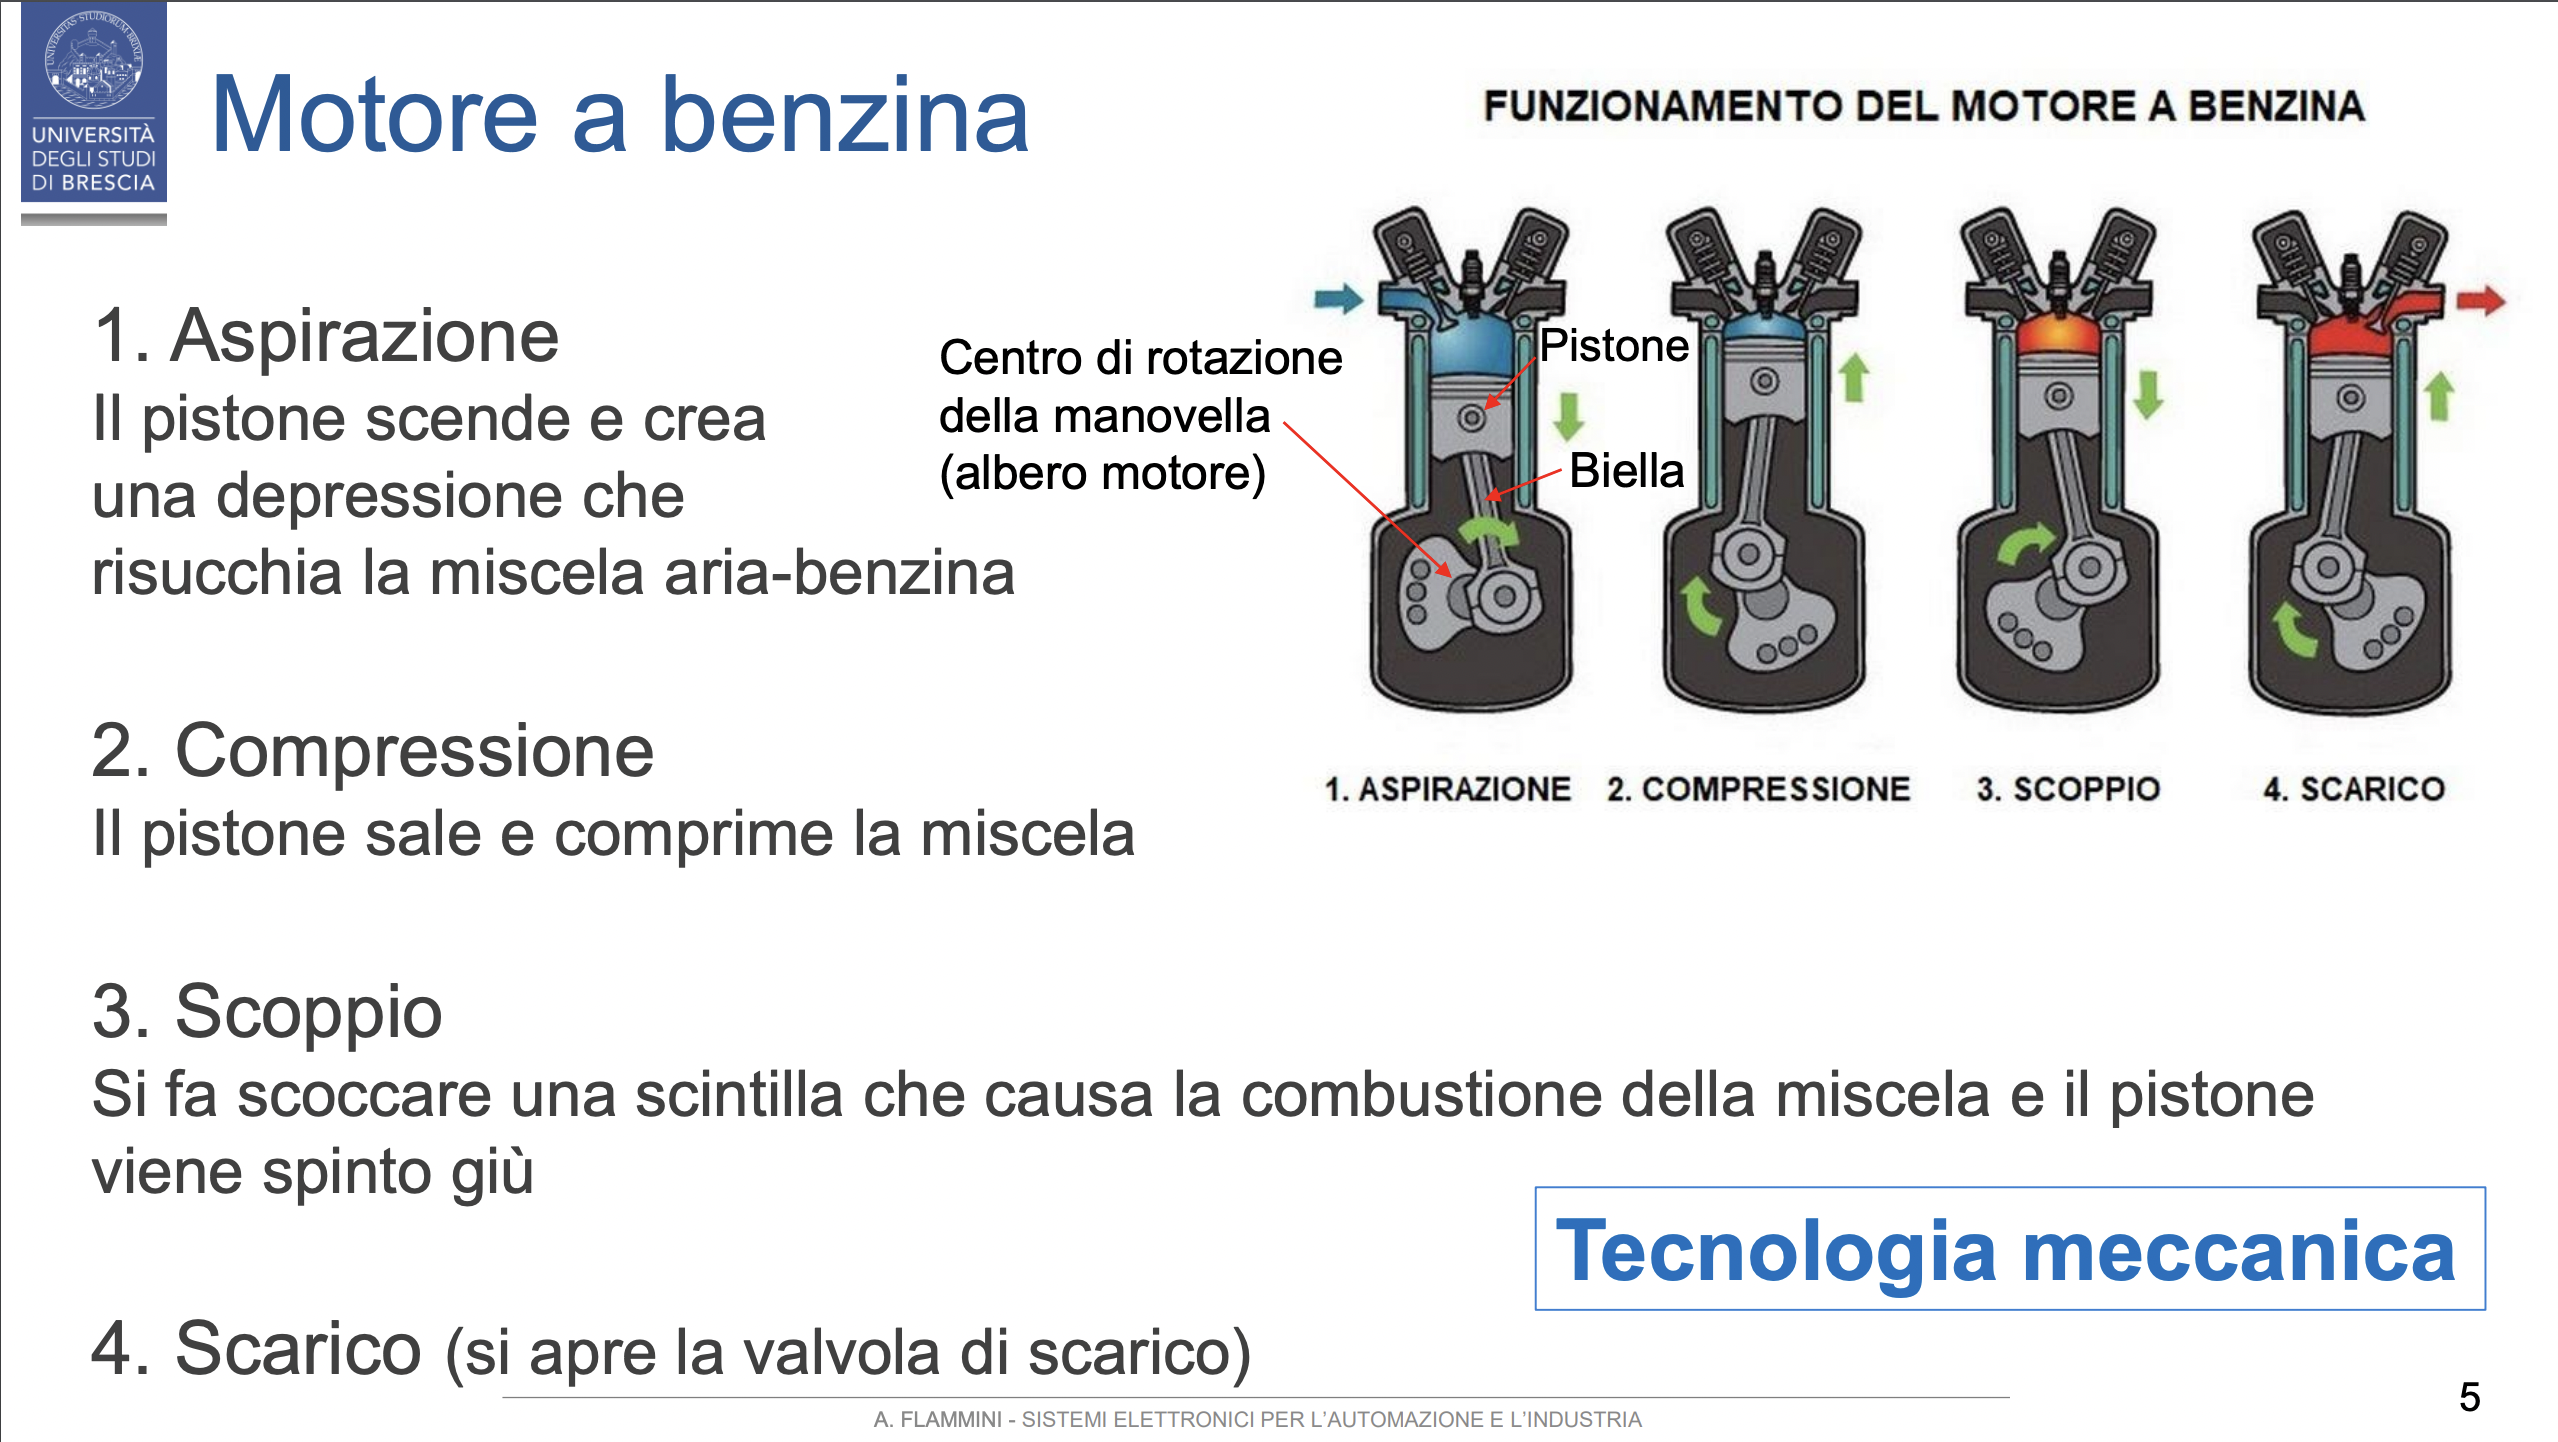
\includegraphics[width=0.7\linewidth]{banz.png}
    \caption{Motore a benzina}
\end{figure}

\subsection{Rivoluzioni industriali}
\begin{figure}[h!]
    \centering
    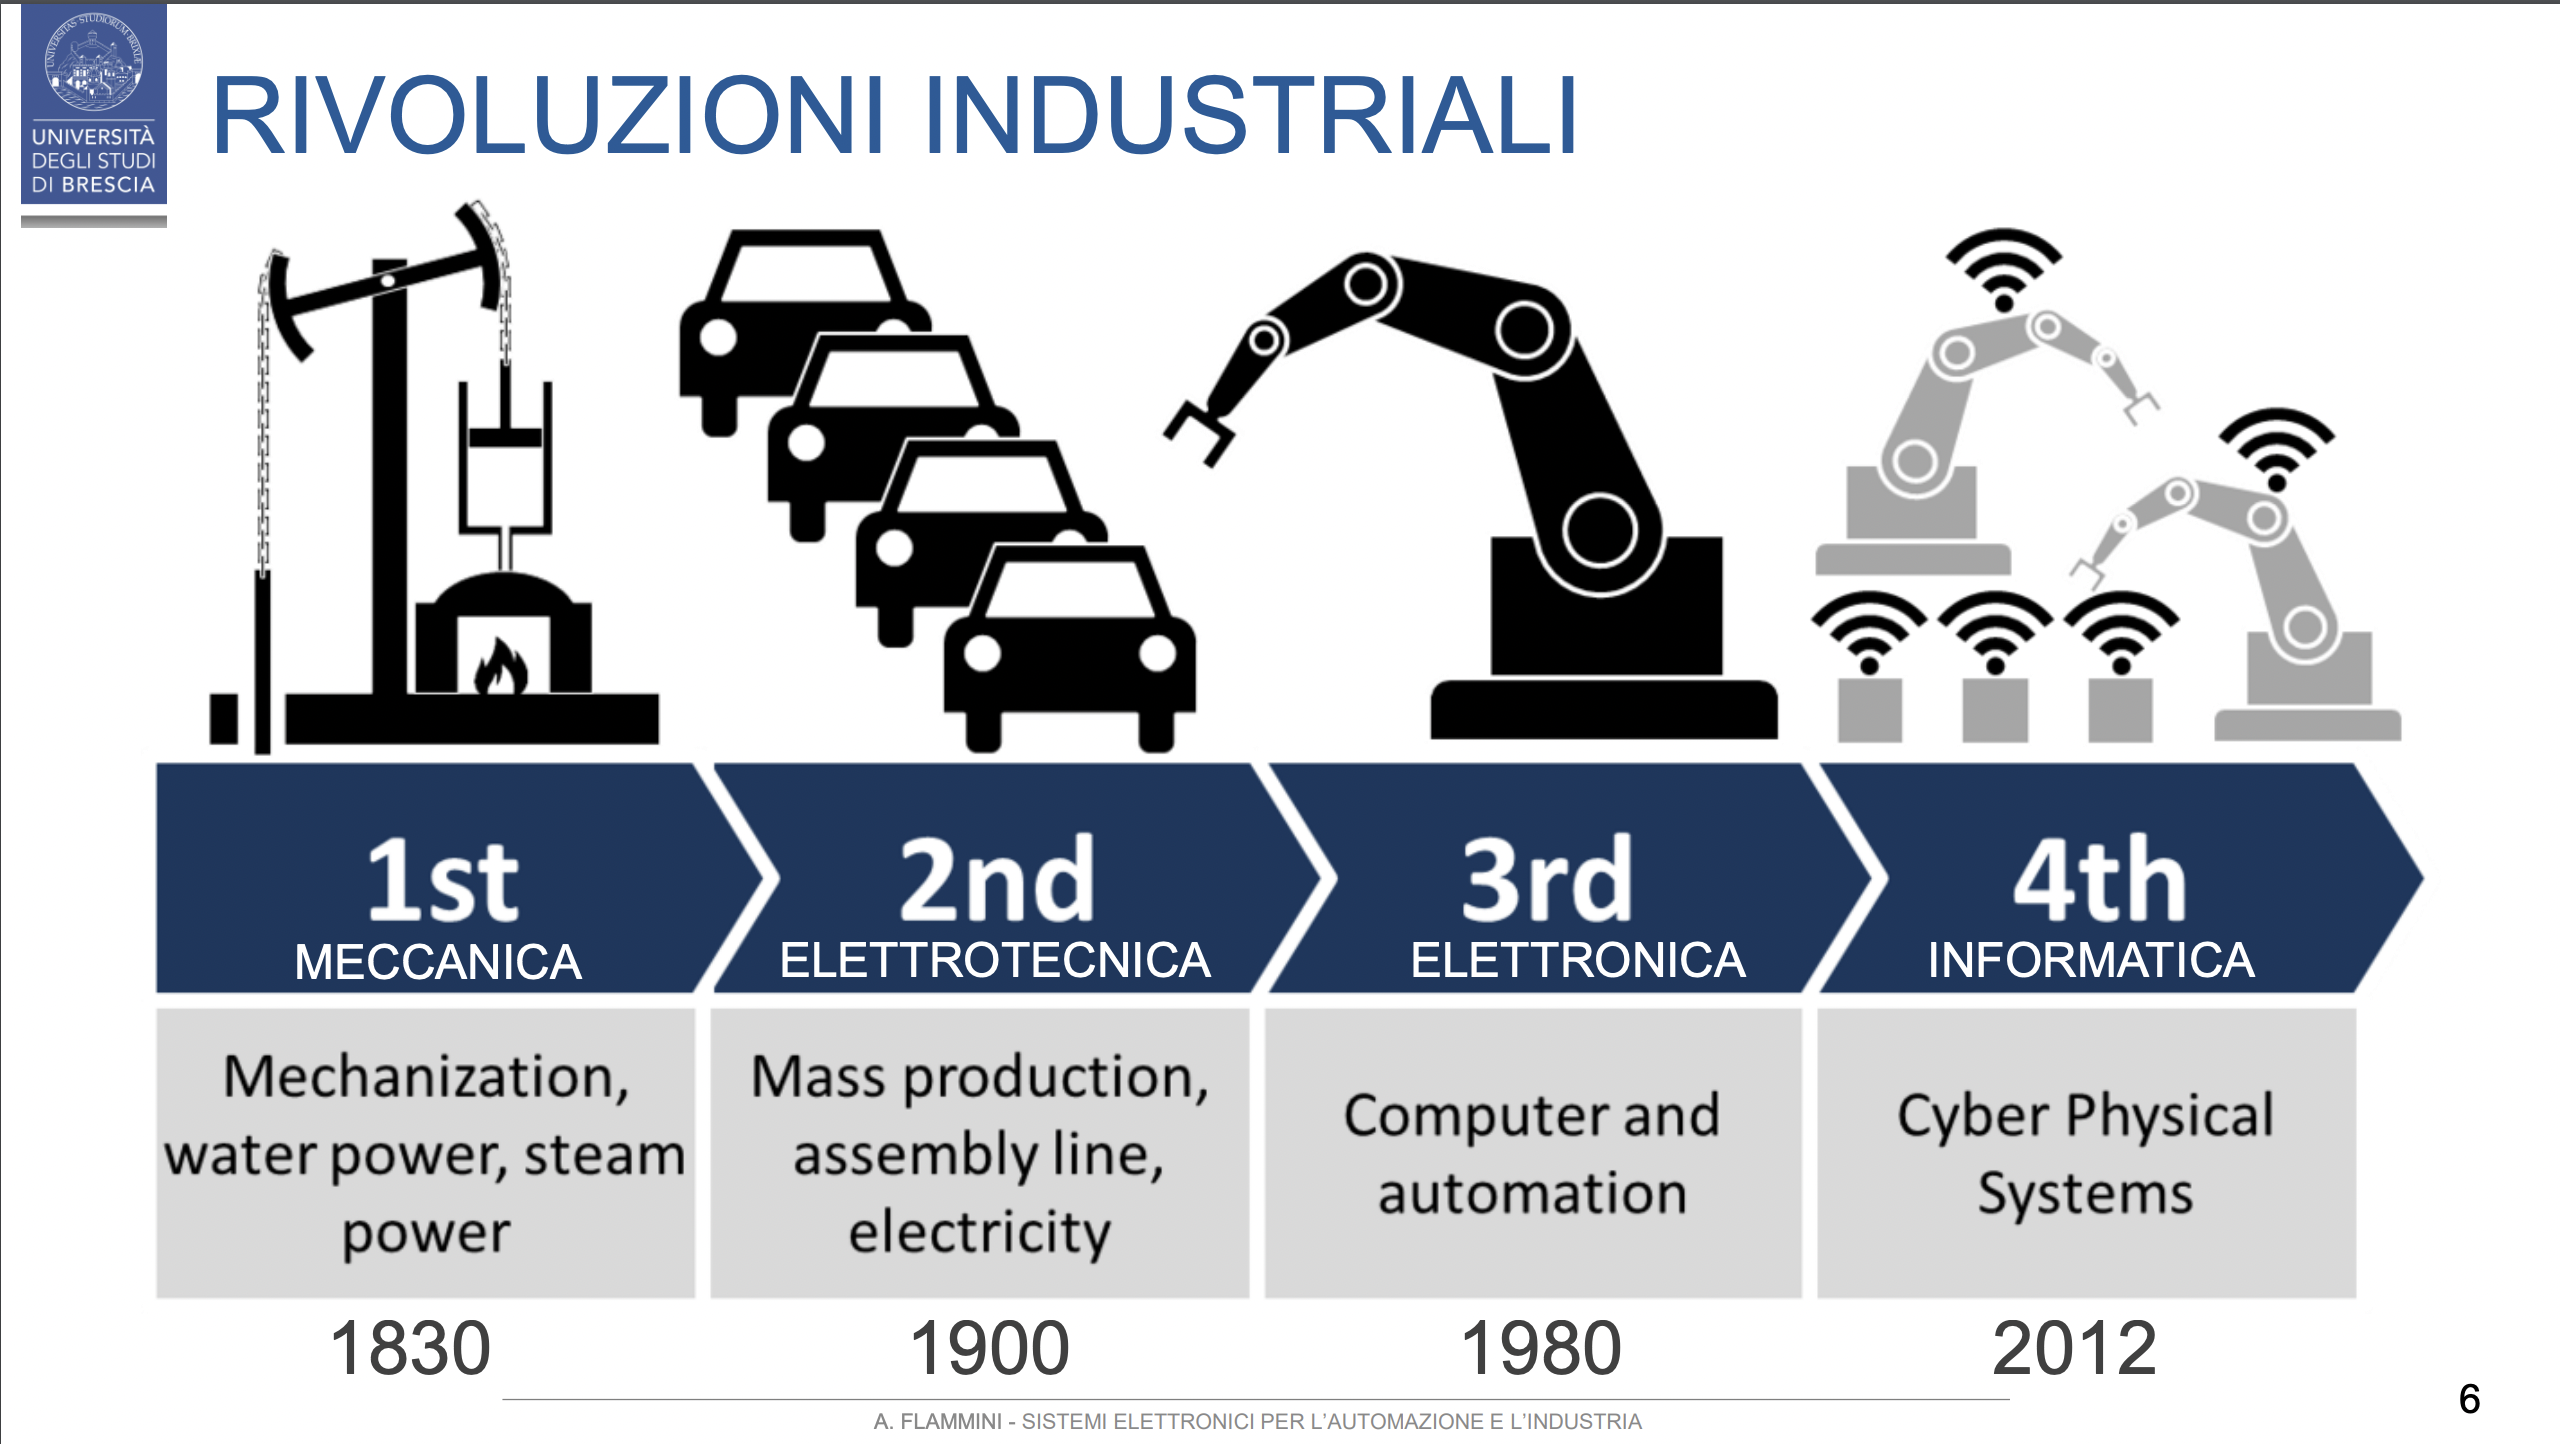
\includegraphics[width=0.7\linewidth]{riv.png}
    \caption{Rivoluzioni industriali}
\end{figure}
Energia muscolare $\rightarrow$ vento, energia naturale $\rightarrow$ forni $\rightarrow$ vapore $\rightarrow$ elettricità, con la quale si avvia la produzione di massa (elettrotecninca - fordismo) $\rightarrow$ elettronica (PLC), nato in Giappone con la Toyota $\rightarrow$ reti di comunicazione che permettono ai diversi controllori di comunicare tra di loro $\rightarrow$ informatica (controllo a distanza) $\rightarrow$ quinta rivoluzione industriale, rivolzione umano-centrica, impone una grandissima attenzione all'ambiente; l'impatto ambientale della produzione negli ultimi 10 anni è uno dei punti focali - controlli sulle proprie emissioni. Il consumo di elettricità, gas e acqua è un problema, ma il consumo più elevato riguarda l'acqua (sopratutto alimentari) e il più grande problema è che non si sappia come smaltirla.

\subsection*{Classificazione a 3 assi dei sistemi di produzione}
\begin{itemize}
    \item \textbf{Asse del mercato}: modalità di vendita, su ordine (progetta, produci, assembla) per il magazzino (previsione)
    \item \textbf{Asse gestionale}: modalità di realizzazione del volume. Produzioni unitario su commessa, a lotti, continue. 
    \item \textbf{Asse tecnologico}: modalità di realizzazione del prodotto. \begin{itemize}
        \item Industria di base o di processo: produzione di energia, processi chimici, processi estrattivi. Industria che riguarda la distribuzione
        \item Industria di fabbricazione: produzione da materiali grezzi o semilavorati (\textbf{irreversibile} - trasformazione fisico-tecnica) e assemblaggio (tendenzialmente \textbf{reversibile}).
    \end{itemize}
\end{itemize}

\section{Impianti di processo e di fabbricazione}
\subsection*{Impianto industriale}
"Insieme di capitali, macchine, mezzi e addetti atti a utilizzare le risorse materiali ed
energetiche per trasformarle in prodotti finiti a maggior valore aggiunto attraverso
trasformazioni chimico fisiche e/o processi di fabbricazione e/o montaggio".\\
E' fondamentale nella realizzazione del prodotto diminuire il suo peso.\\
\textbf{Time to market} problema notevole: tempo che intercorre tra la realizzazione del prodotto e la sua commercializzazione.
\subsection{Impianti di processo}
Tanta energia e capitali, sicurezza (safety), affidabilità. Poche grosse aziende che si occupano dell'automazione degli impianti di processo. Capitali enormi e un sacco di persone per aprire un impianto di processo. L'impianto di processo è vasto e complesso. E' un mercato a parte.\\
\textbf{Revamping}: rinnovare la parte obsoleta dell'impianto.\\
La sicurezza è un punto chiave rispetto alle fabbriche.\\ Negli impianti di processo non vengono usati robot in quanto sono bravi (sono molto precisi) a fare una cosa sola, mentre negli impianti di fabbricazione vengono usati. Negli impianti di processo vengono utilizzati gli operai.\\
\subsection{Impianti di fabbricazione}
Basso costo, elevata qualità (pochi scarti), flessibilità.
Spazio all'informatica nelle fabbriche per la \textbf{riduzione delle tolleranze}.\\
Il costo di produzione è basso se uso materie prime non troppo di qualità e lo riesco a produrre in pochissimo tempo, per realizzarne tantissimi in un lasso di breve tempo.

\newpage
\subsection{Processo di produzione}
\begin{figure}[h!]
    \centering
    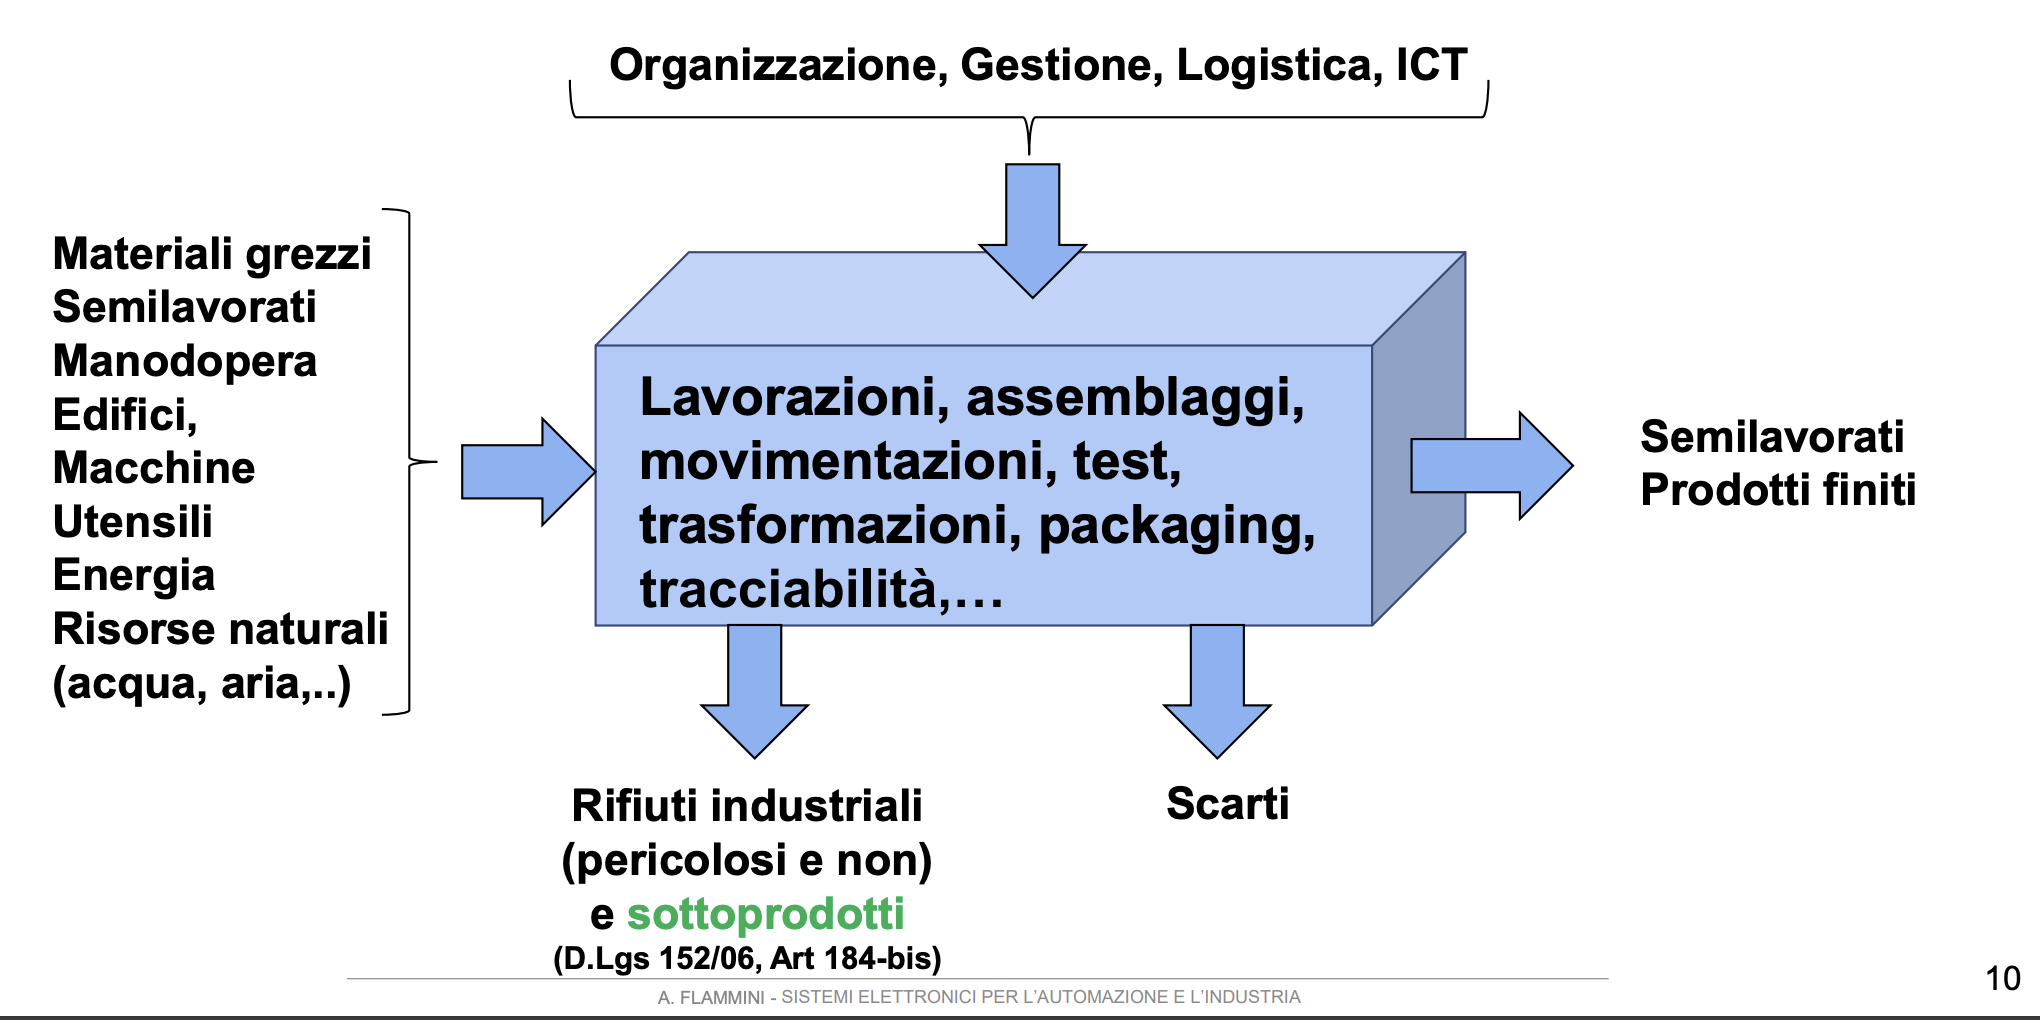
\includegraphics[width=0.6\linewidth]{processo.png}
    \caption{Processo di produzione}
\end{figure}
Dai rifiuti si cerca sempre di ottenere dei sotto-prodotti.\\
Gli scarti posso essere recuperati oppure no, dipende dal costo del prodotto.\\

\subsection{Processi e impianti produttivi}
\begin{figure}[h!]
    \centering
    \begin{minipage}[b]{0.45\textwidth}
        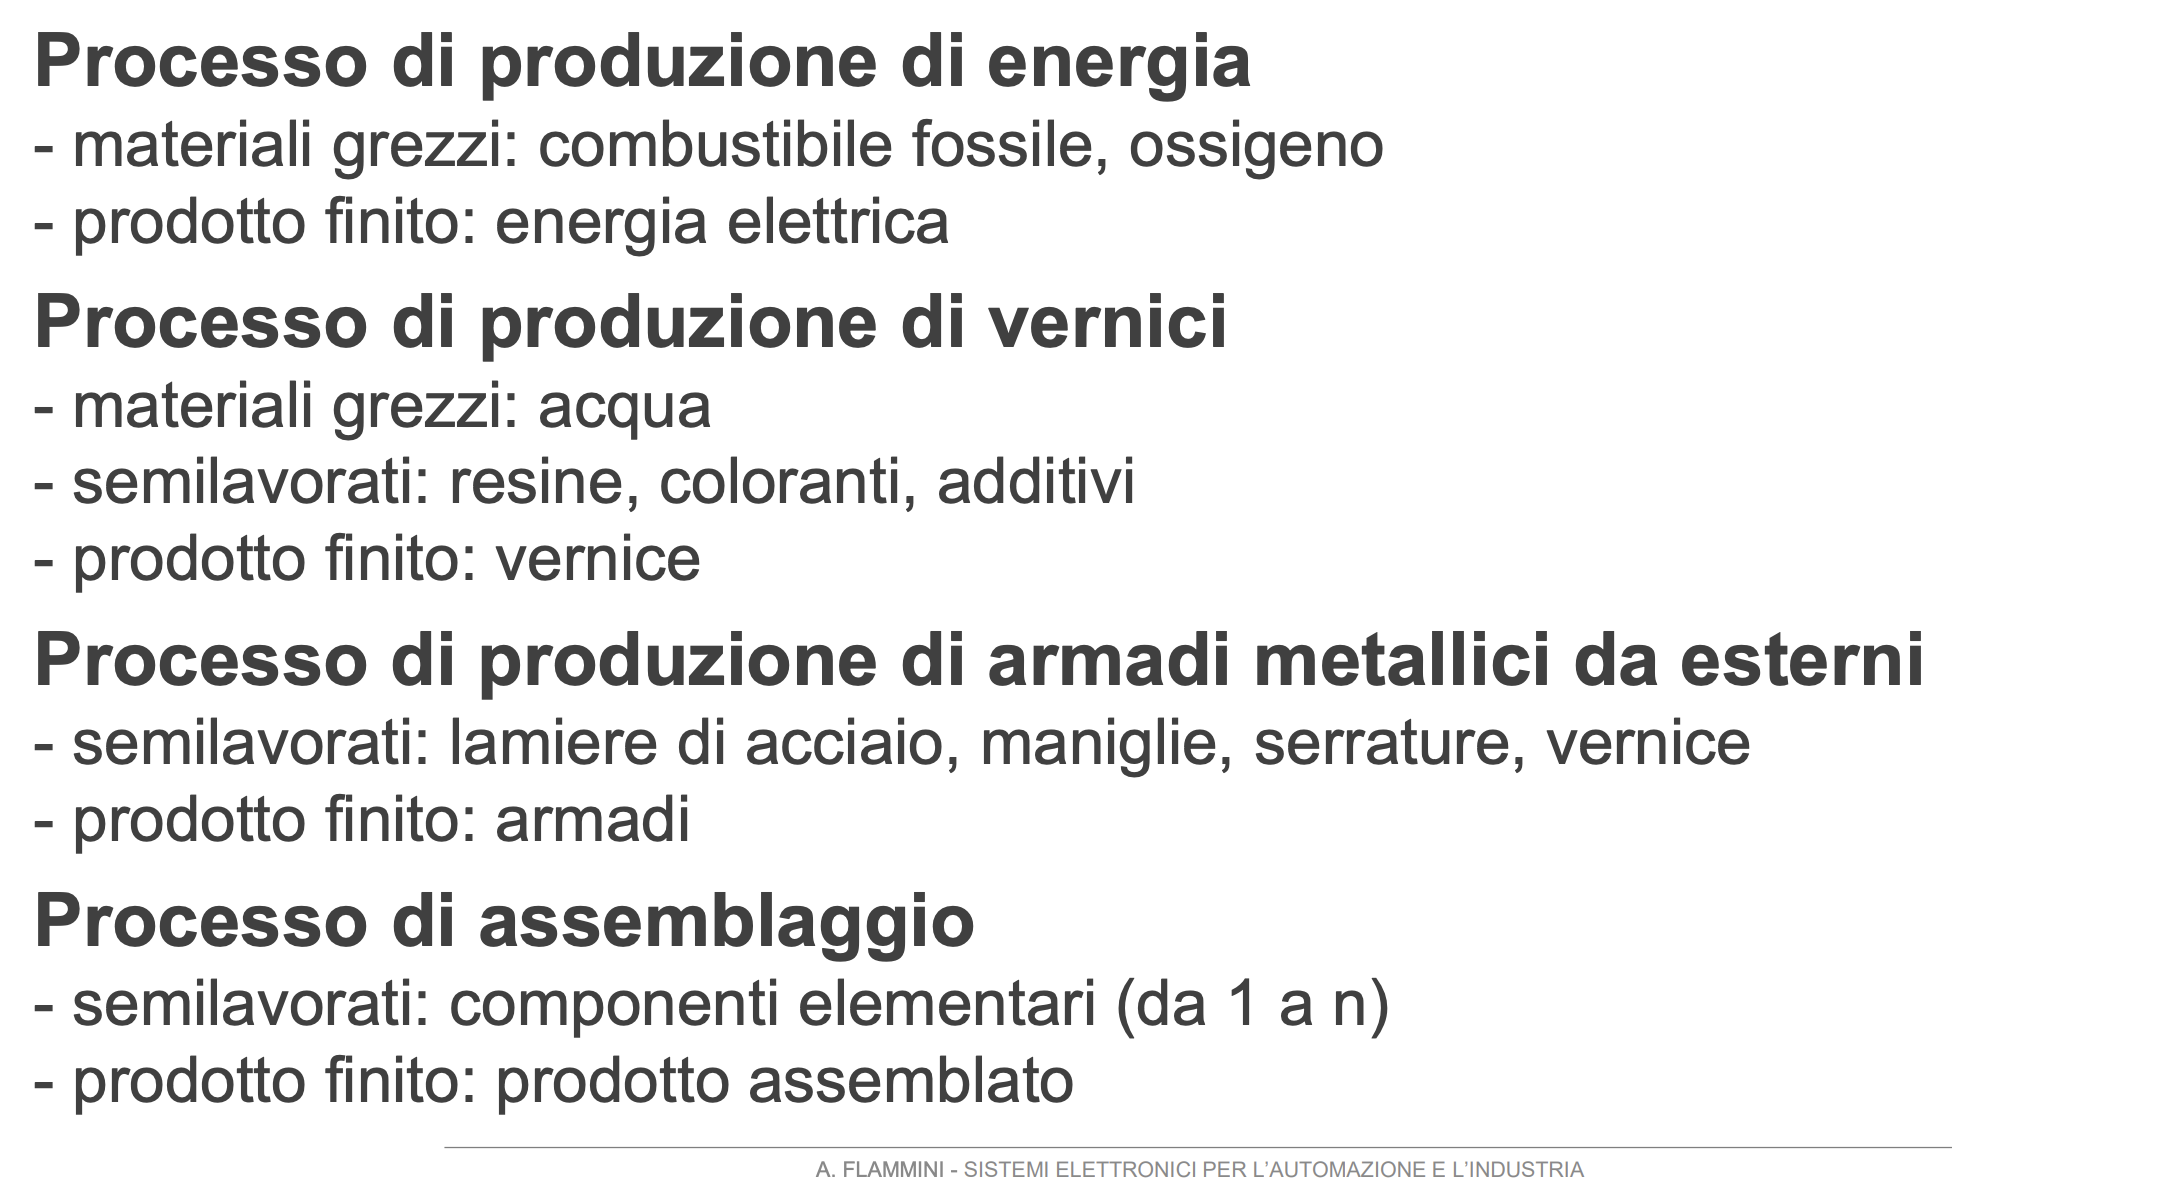
\includegraphics[width=\textwidth]{processieimpianti.png}
        \caption{Processi produttivi}
    \end{minipage}
    \hfill
    \begin{minipage}[b]{0.45\textwidth}
        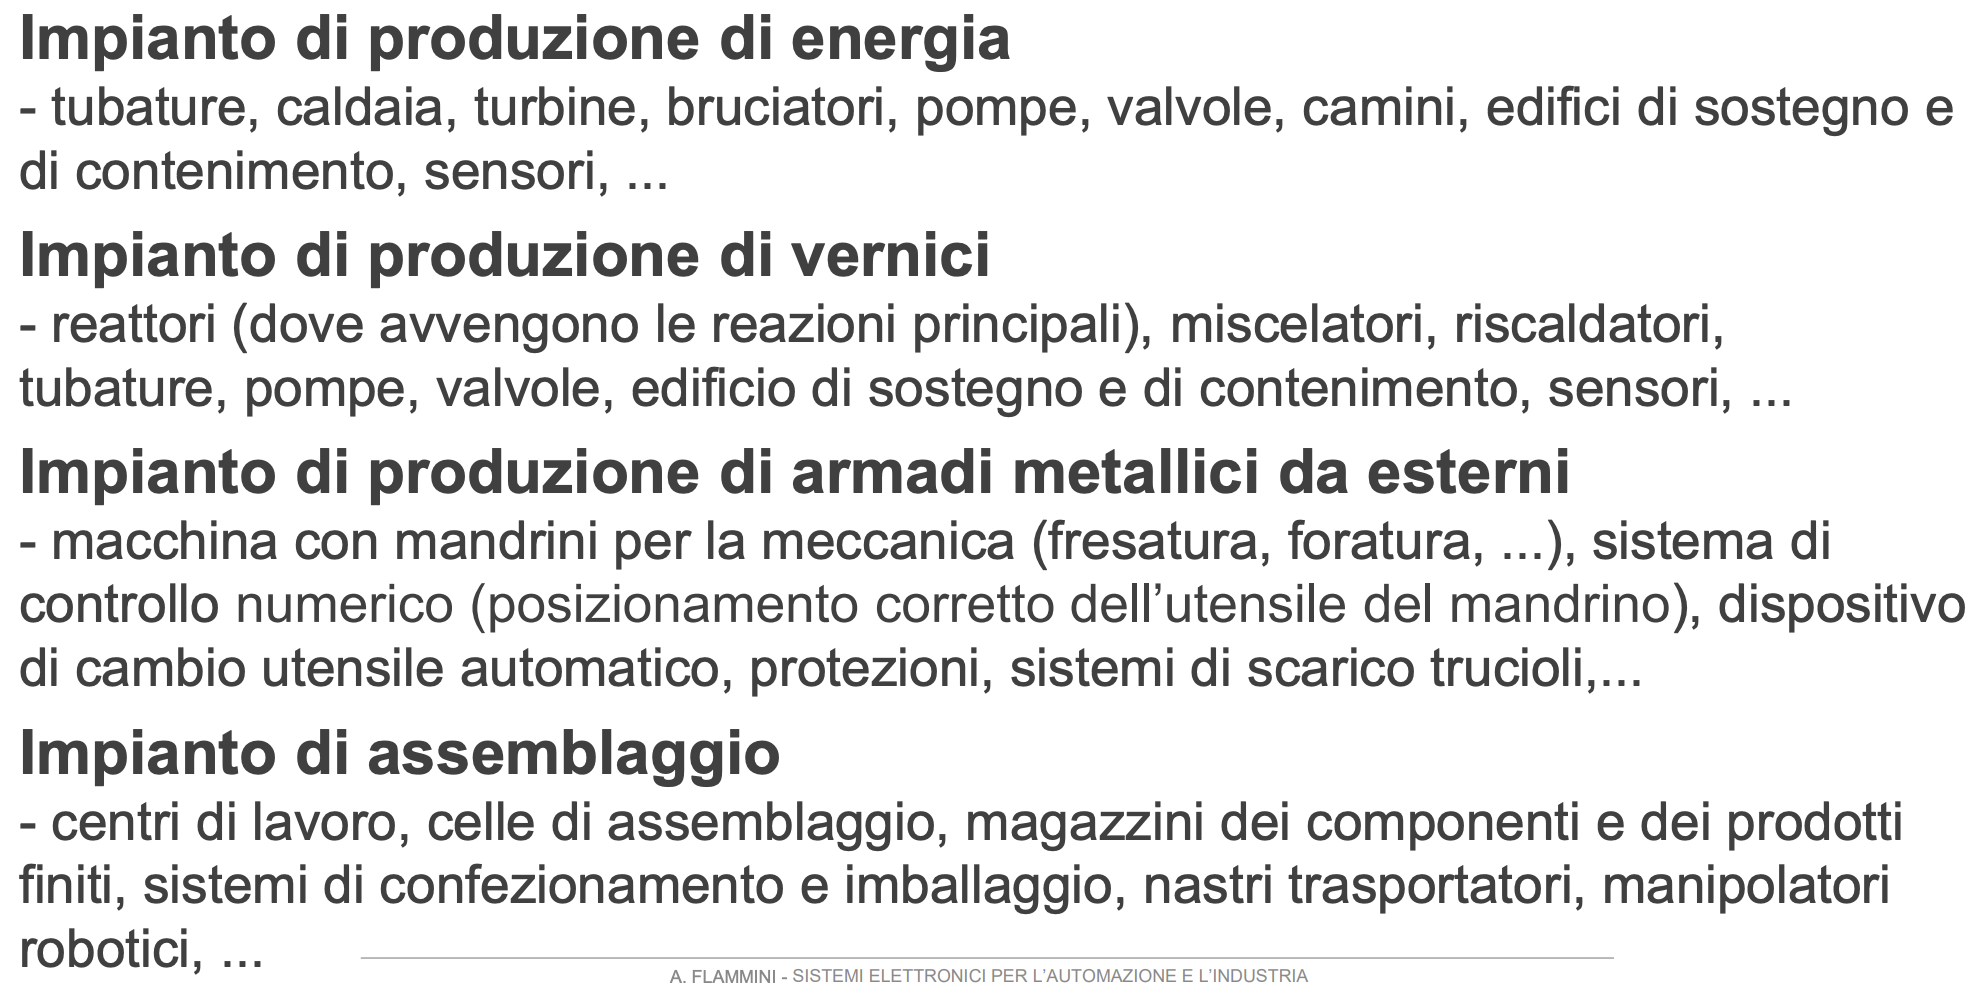
\includegraphics[width=\textwidth]{processieiimpianti2.png}
        \caption{Impianti produttivi}
    \end{minipage}
\end{figure}

\subsection{Automazione Industriale}
\begin{figure}[h!]
    \centering
    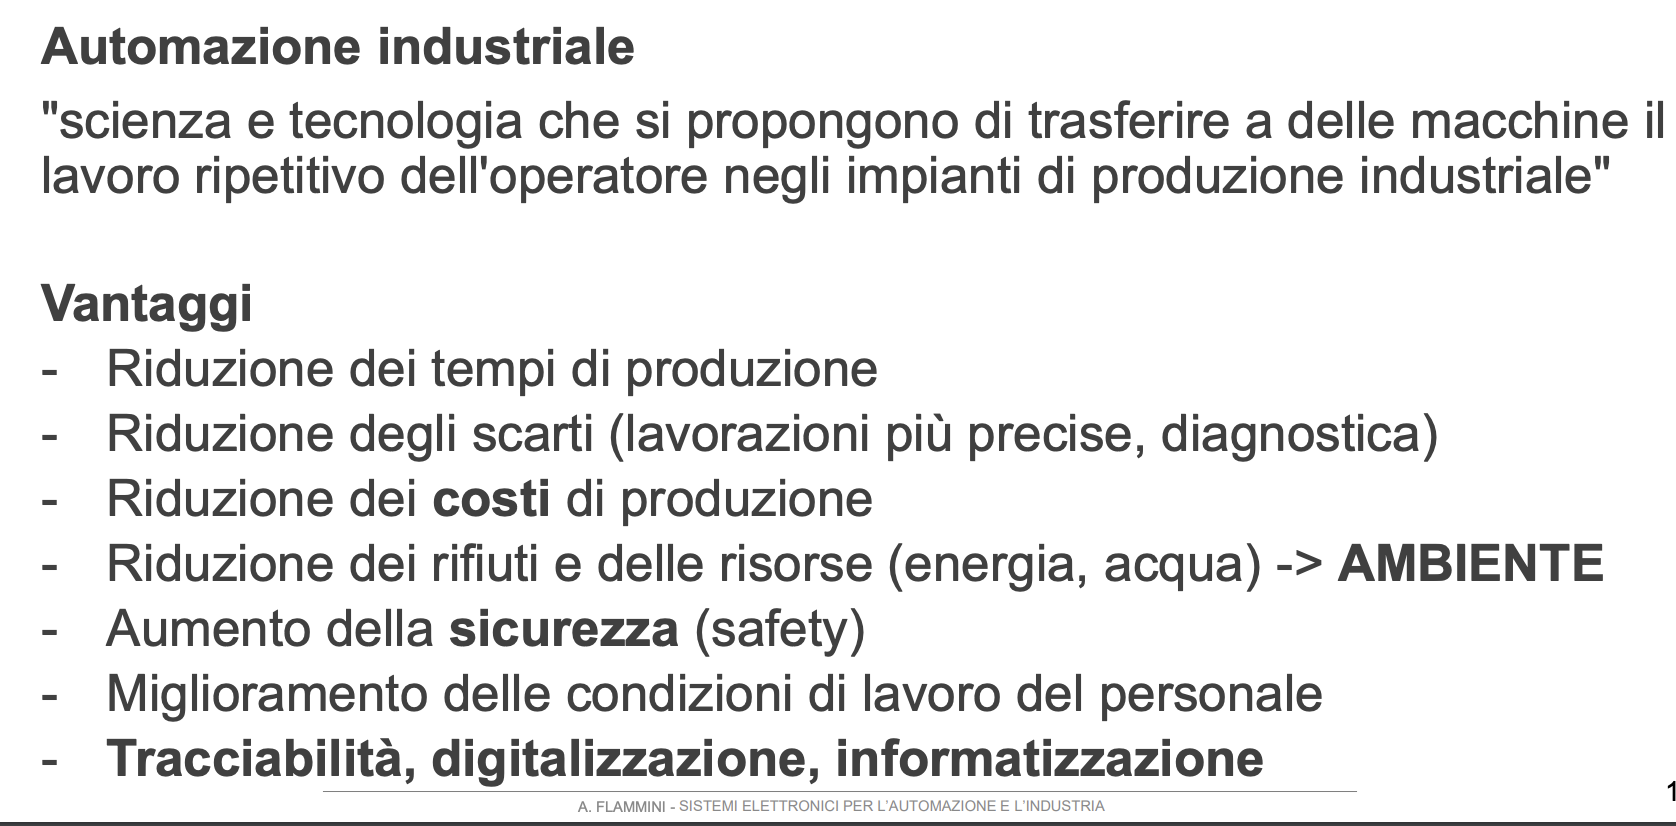
\includegraphics[width=0.5\linewidth]{automazione.png}
    \caption{Automazione industriale}
\end{figure}

\subsubsection{Definizioni}
\begin{figure}[h!]
    \centering
    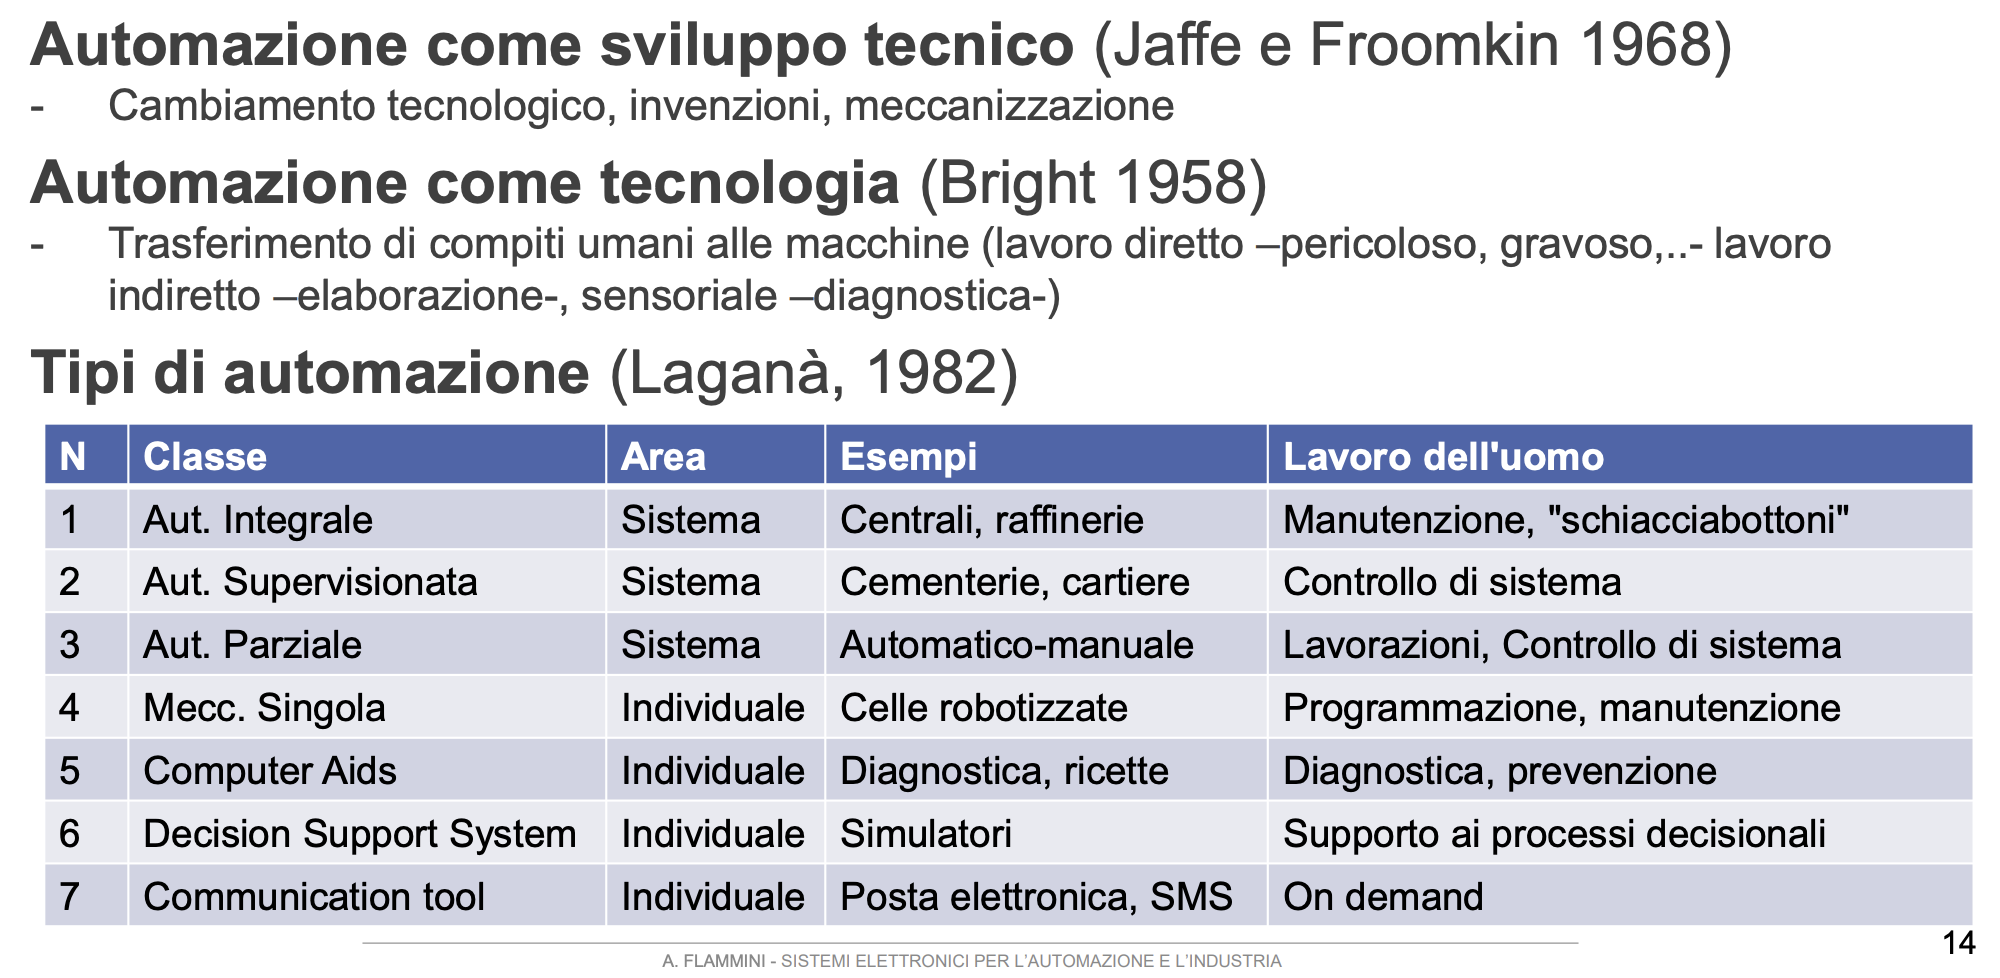
\includegraphics[width=0.5\linewidth]{auto2.png}
    \caption{Definizioni}
\end{figure}

\subsubsection{Terza, Quarta rivoluzione industriale}
\begin{figure}[h!]
    \centering
    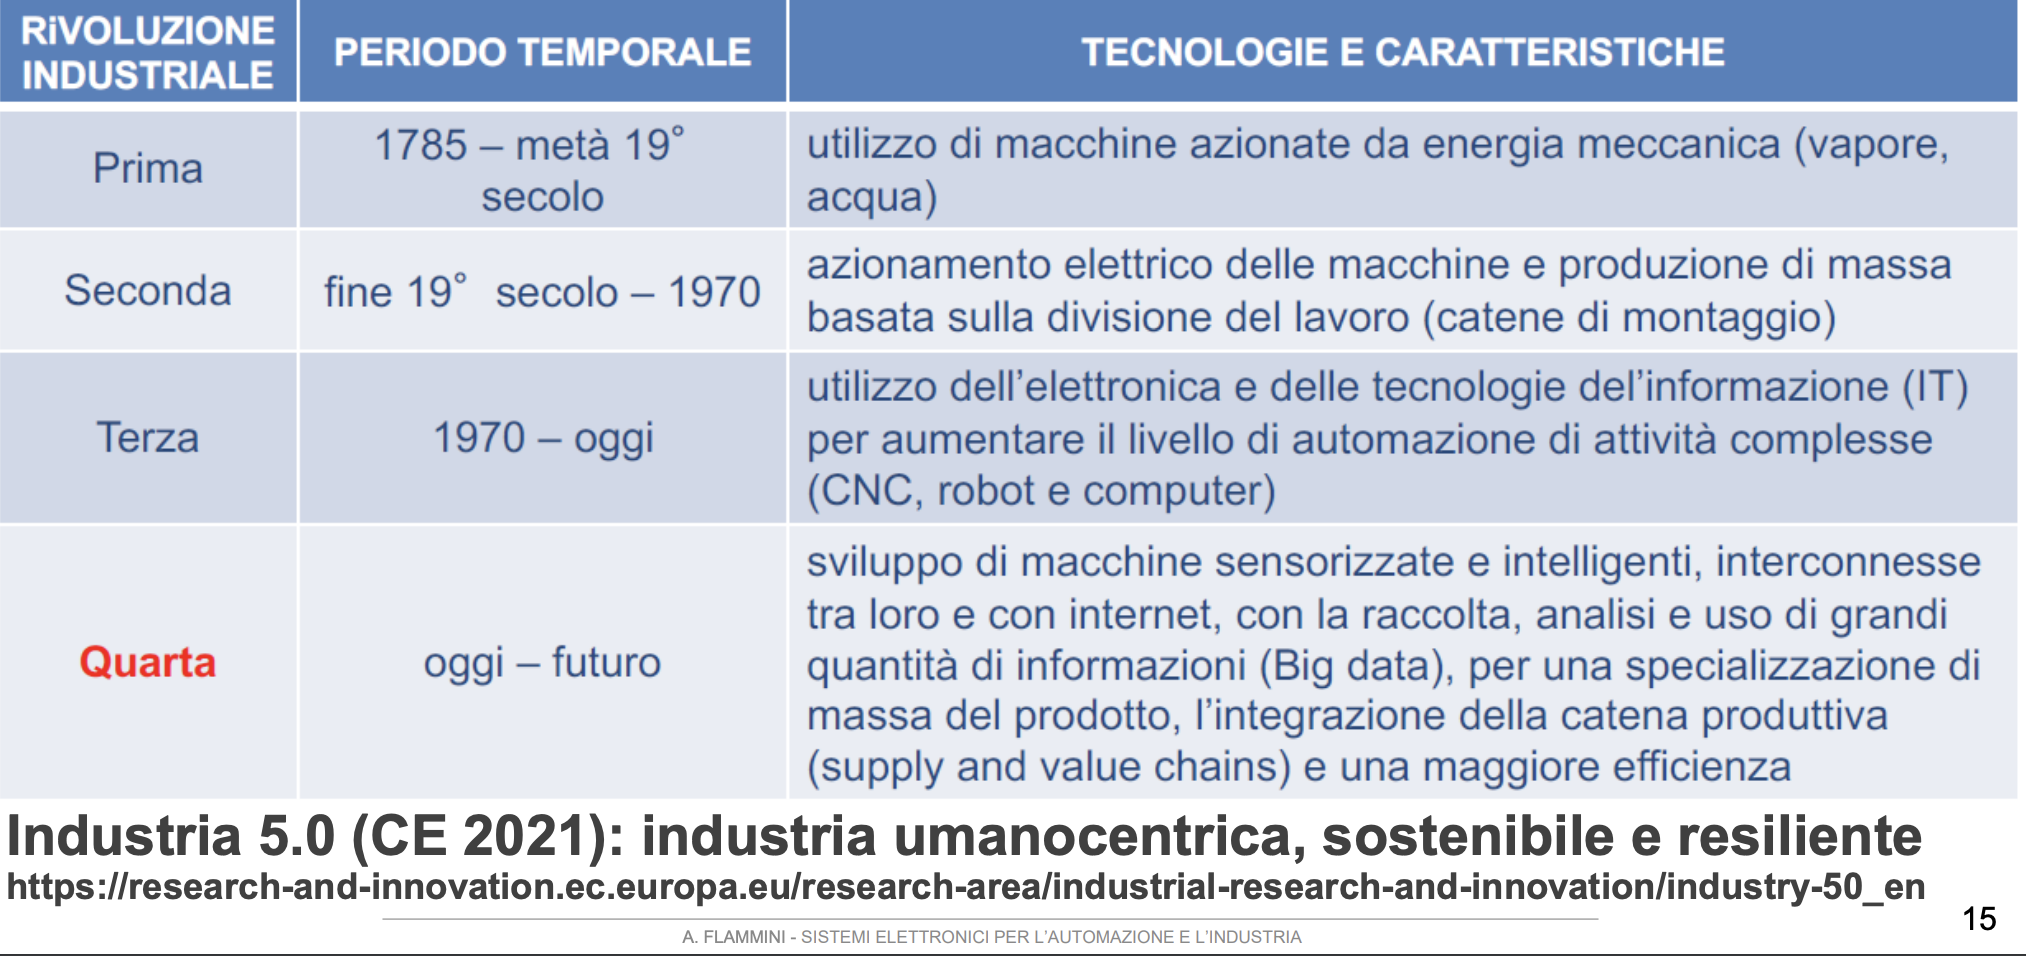
\includegraphics[width=0.5\linewidth]{34.png}
    \caption{Terza, Quarta rivoluzione industriale}
\end{figure}
\textbf{Sostenibile}: ha un basso impatto ambientale.
\textbf{Resilienza}: capacità di un sistema di riprendersi da un evento che lo ha messo in crisi - accettare il cambiamento e adattarsi ad esso.

\subsubsection{Layout}
\begin{figure}[h!]
    \centering
    \begin{minipage}[b]{0.45\textwidth}
        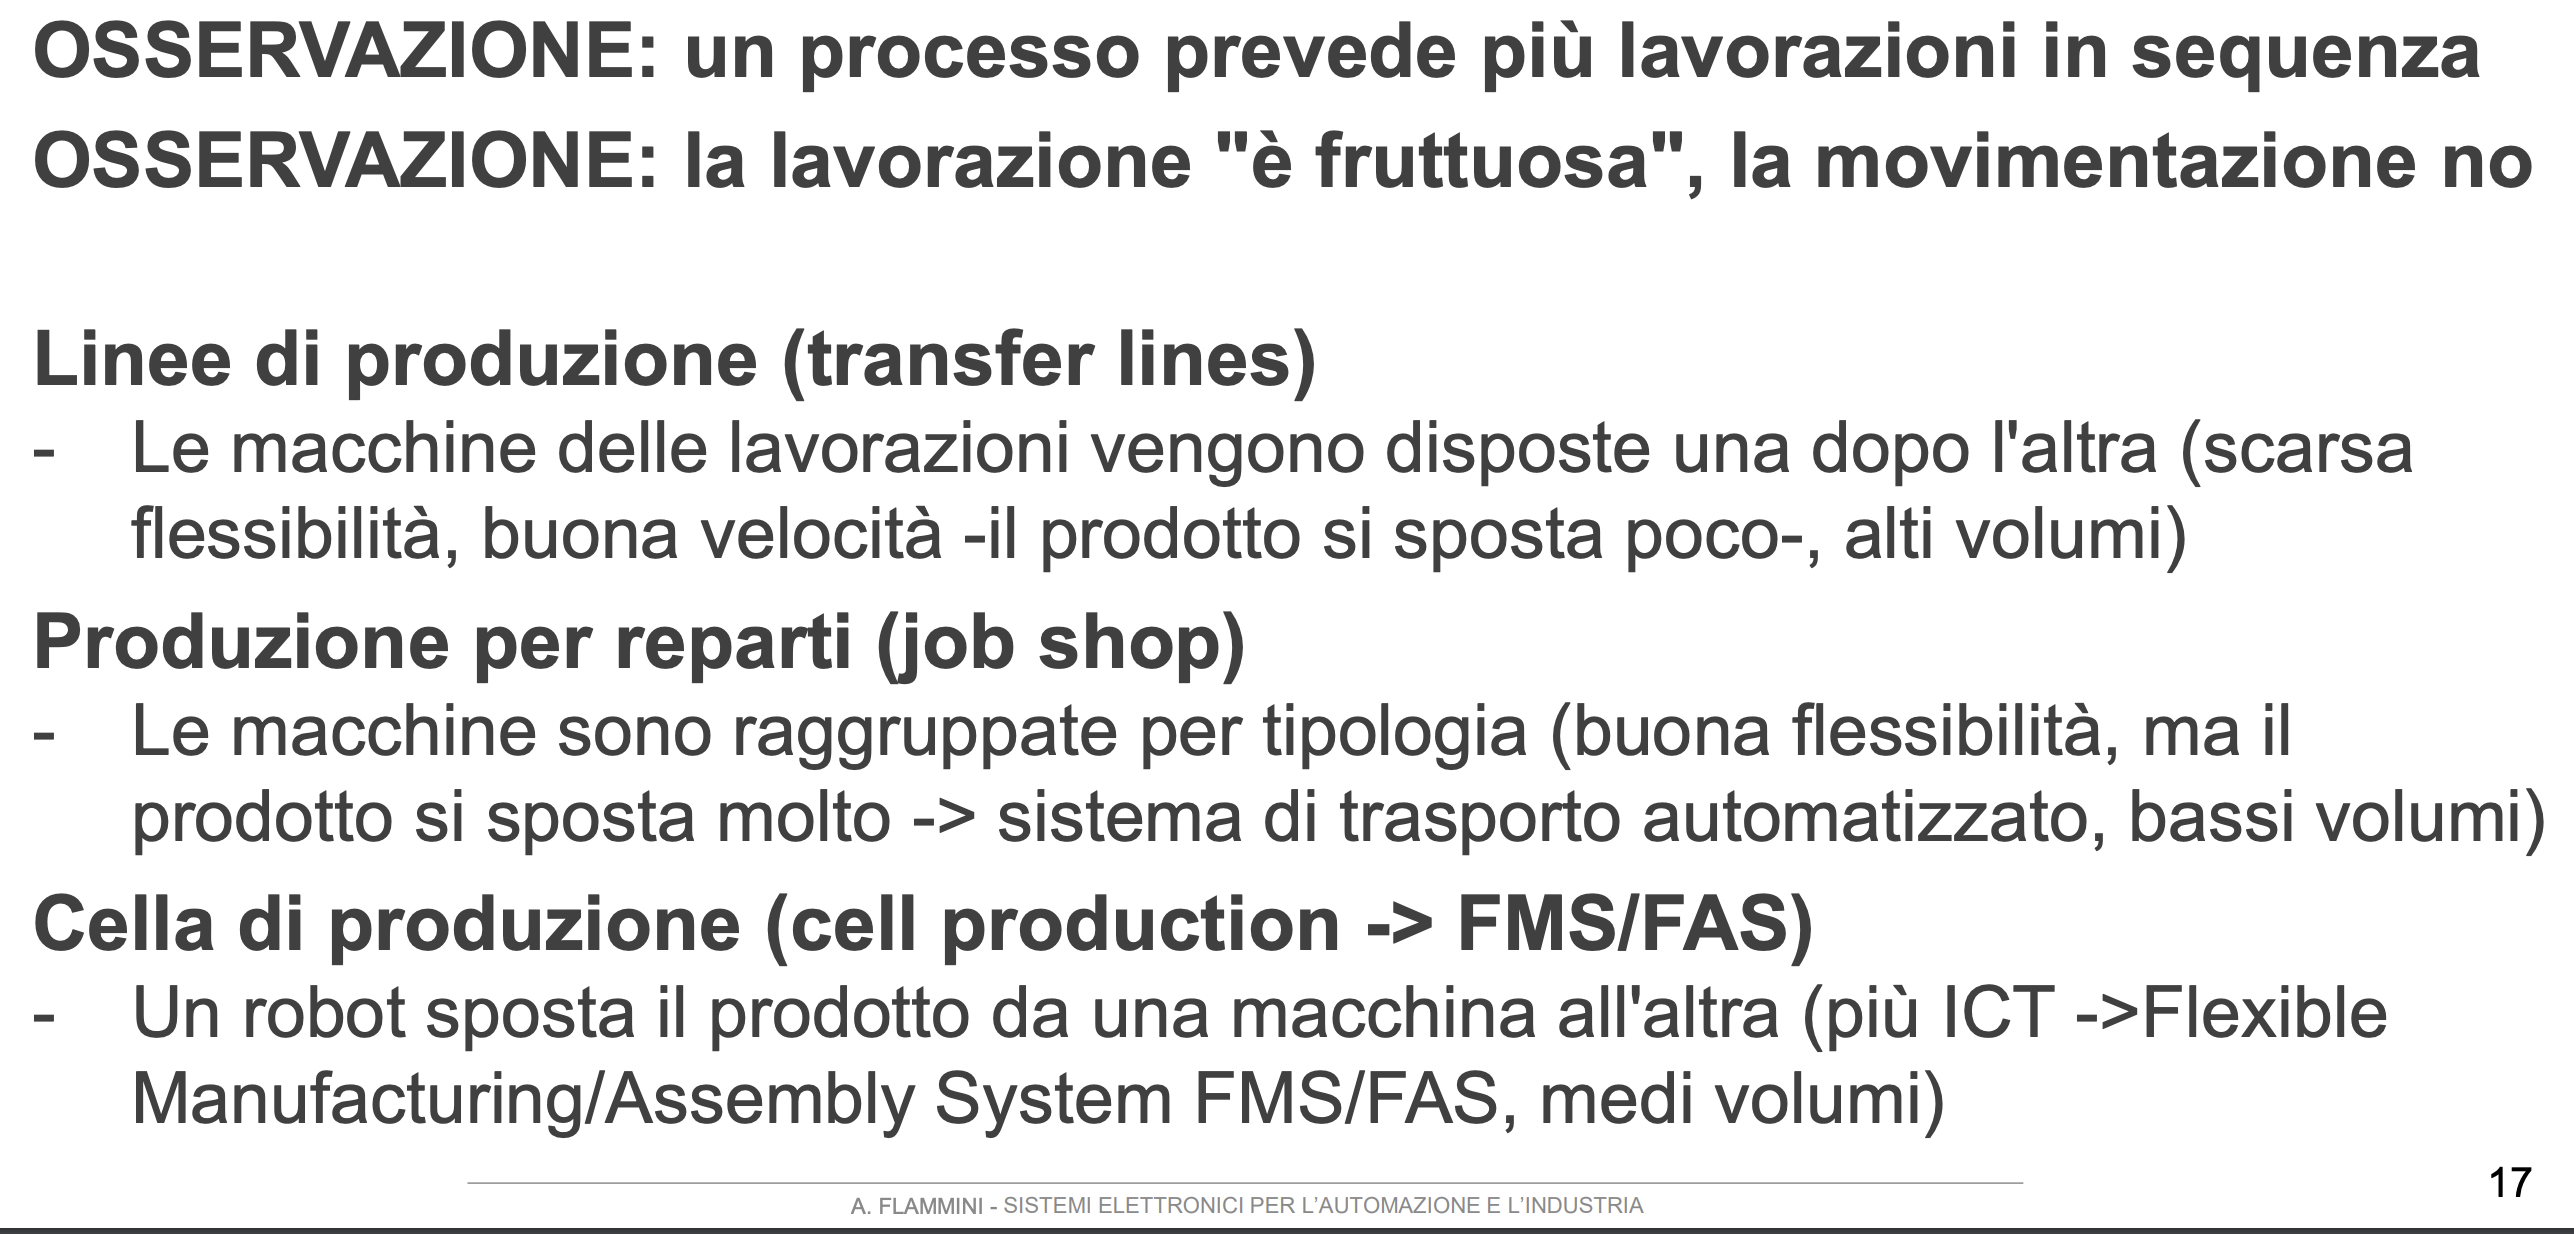
\includegraphics[width=\textwidth]{layout.png}
        \caption{Layout}
    \end{minipage}
    \hfill
    \begin{minipage}[b]{0.45\textwidth}
        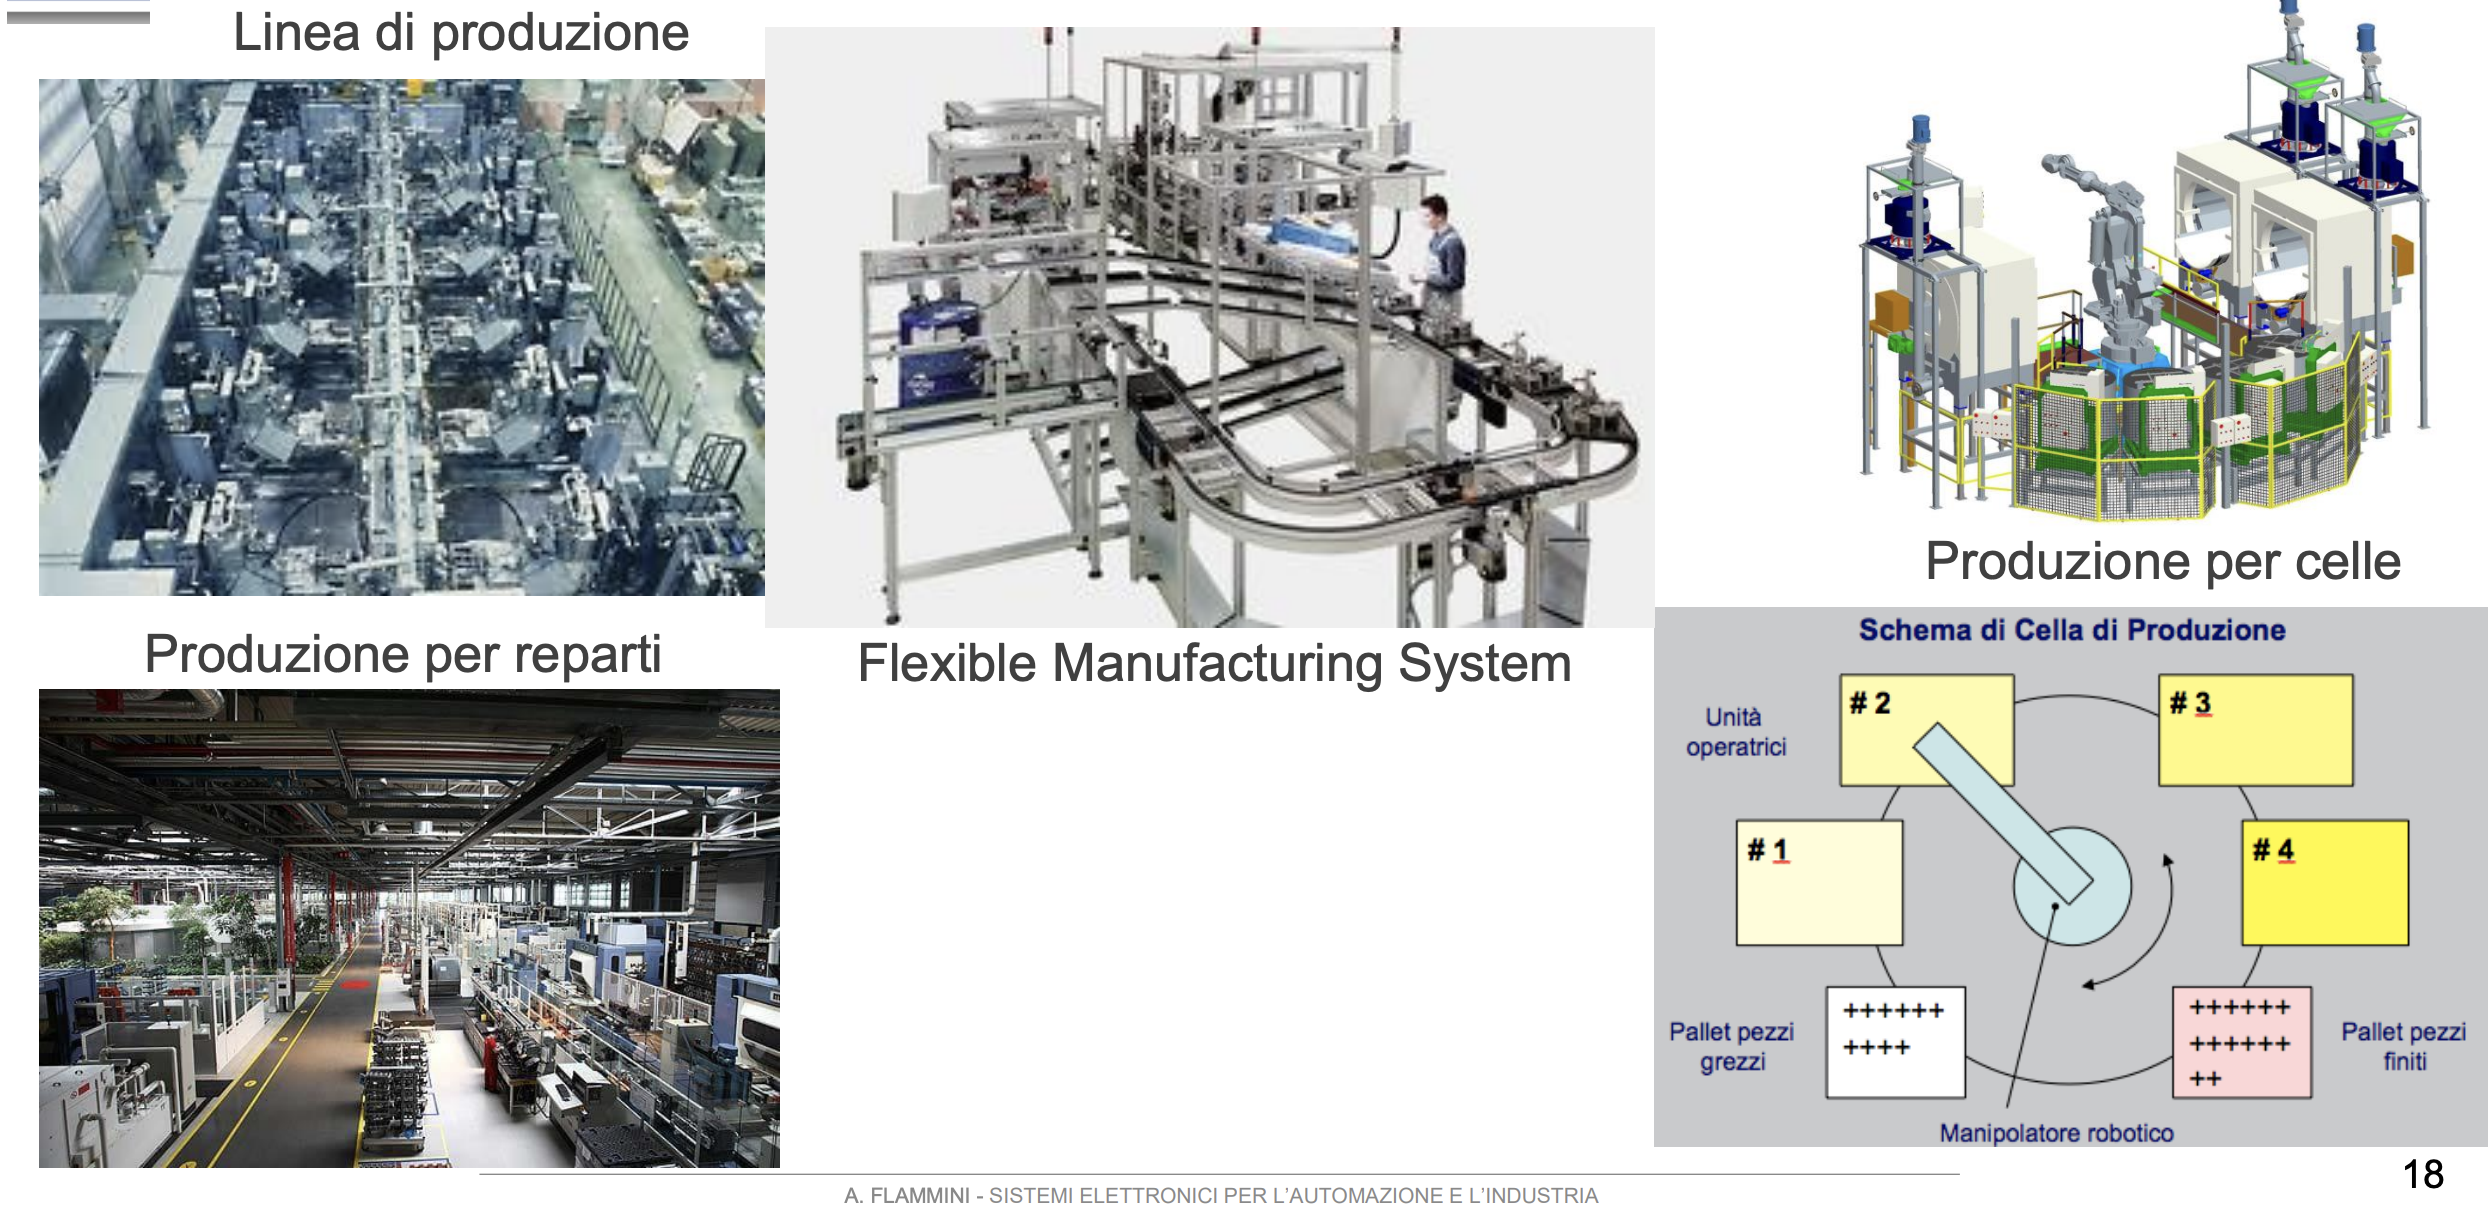
\includegraphics[width=\textwidth]{layout2.png}
        \caption{Layout}
    \end{minipage}
\end{figure}
\textbf{FMS}: Flexible Manufacturing System, automatizzata ma con la presenze dell'operaio.

\newpage
\section{CIM}
\begin{figure}[h!]
    \centering
    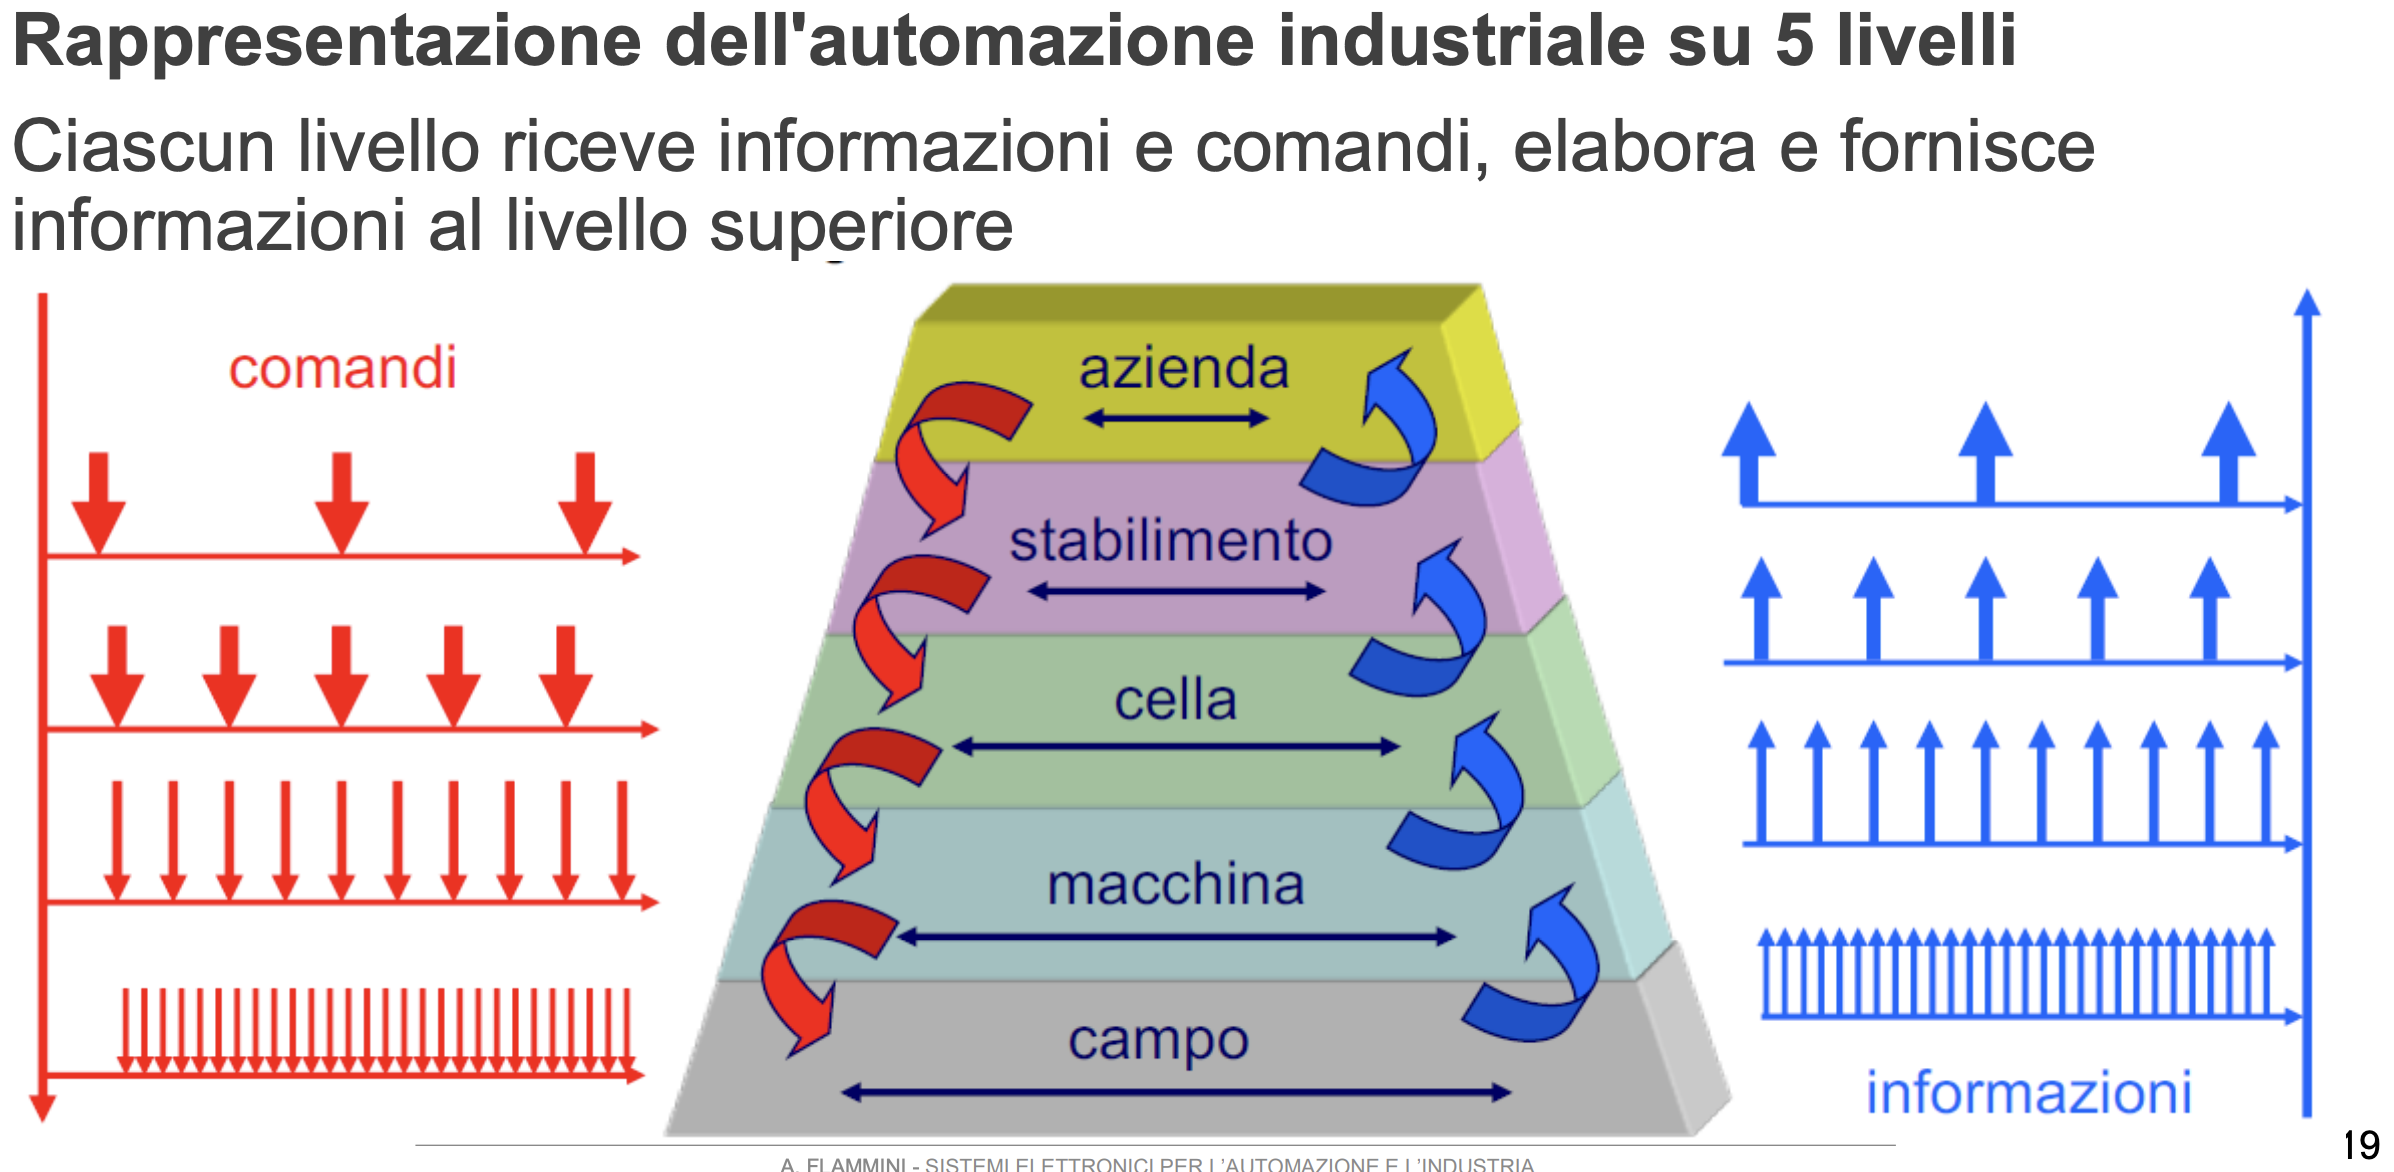
\includegraphics[width=0.5\linewidth]{cim.png}
    \caption{Computer Integrated Manufacturing}
\end{figure}
Le informazioni vengono raggruppate man mano che si passa al livello successivo, mentre i comandi vengono "spacchettati" man mano che si scende di livello.
\begin{figure}[h!]
    \centering
    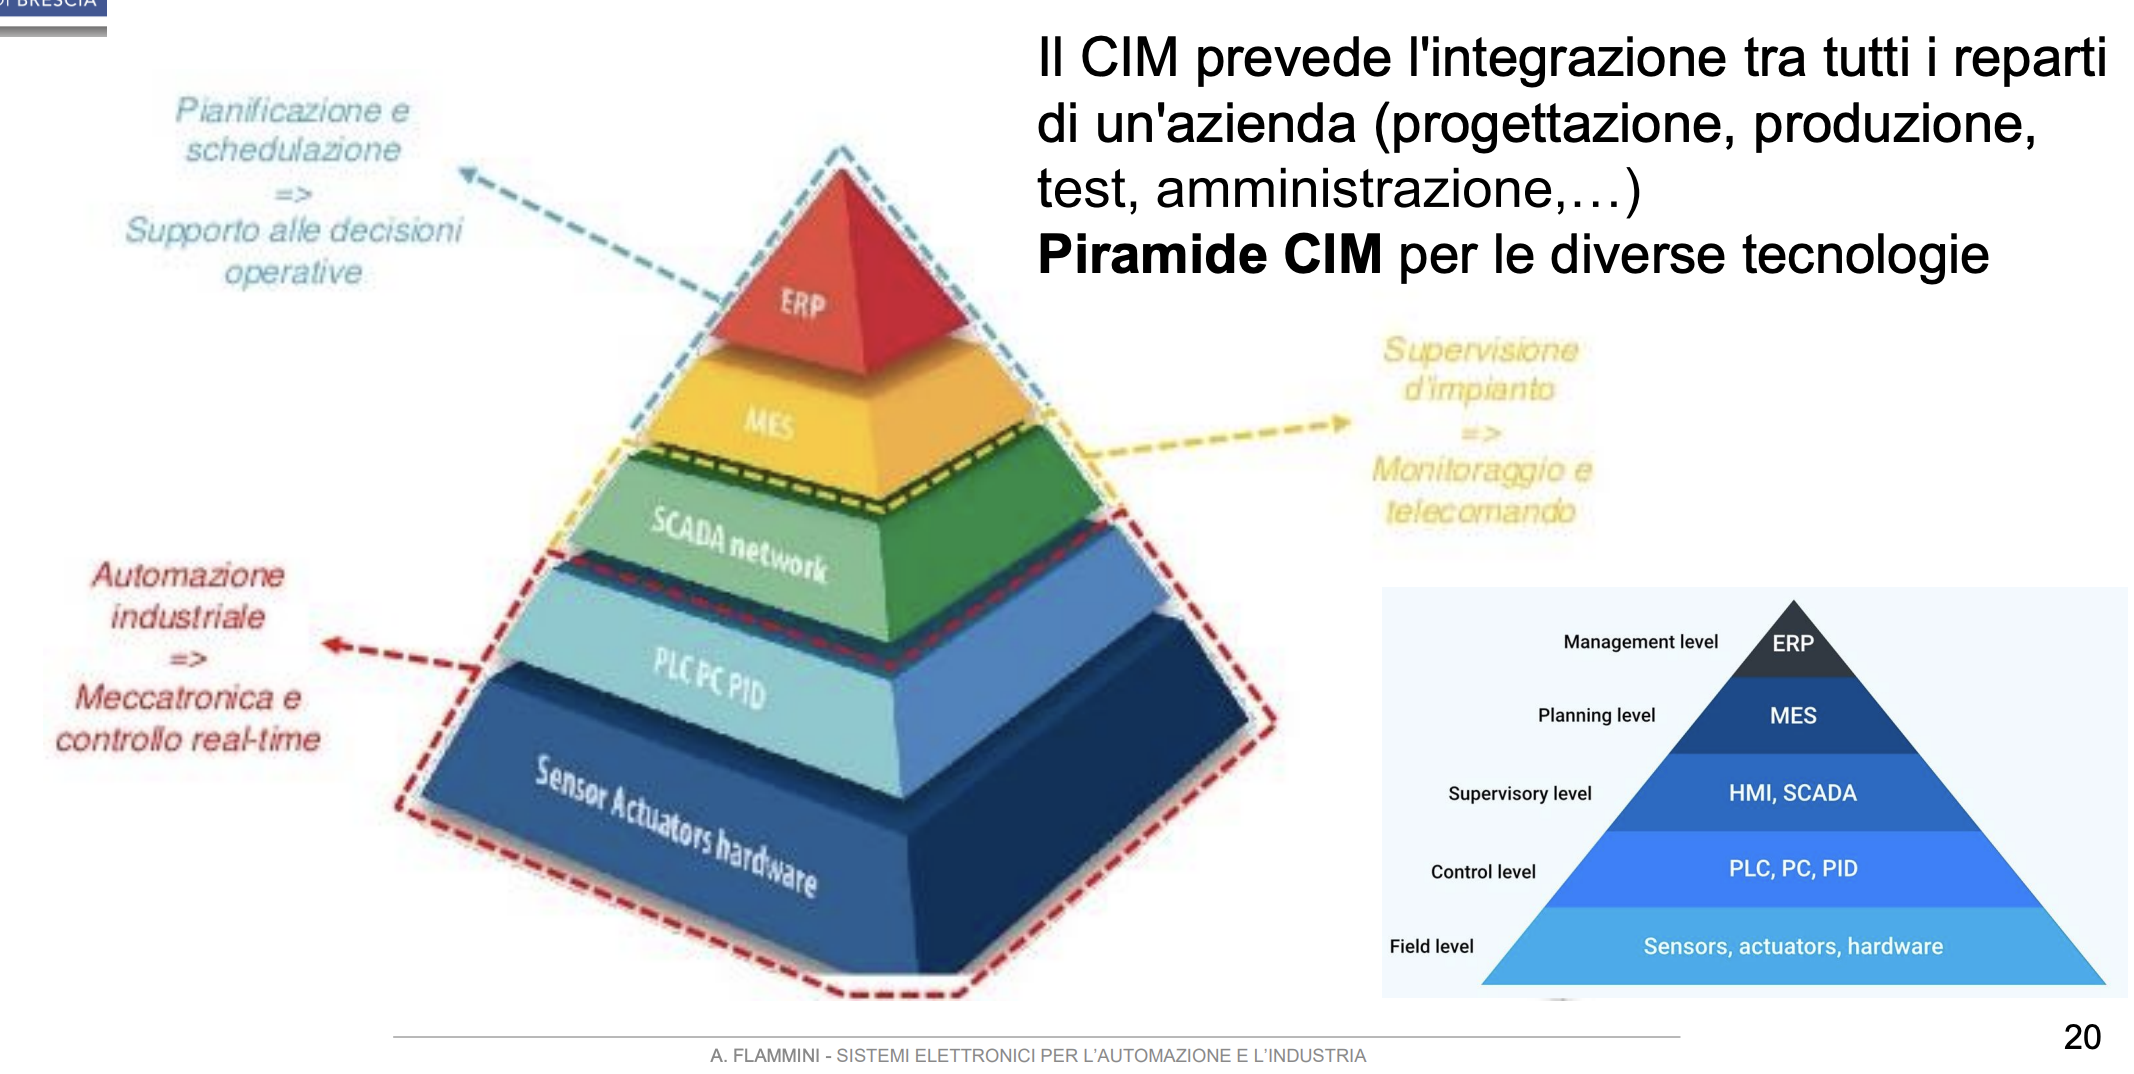
\includegraphics[width=0.5\linewidth]{cim2.png}
    \caption{Computer Integrated Manufacturing}
\end{figure}
\begin{figure}
    \centering
    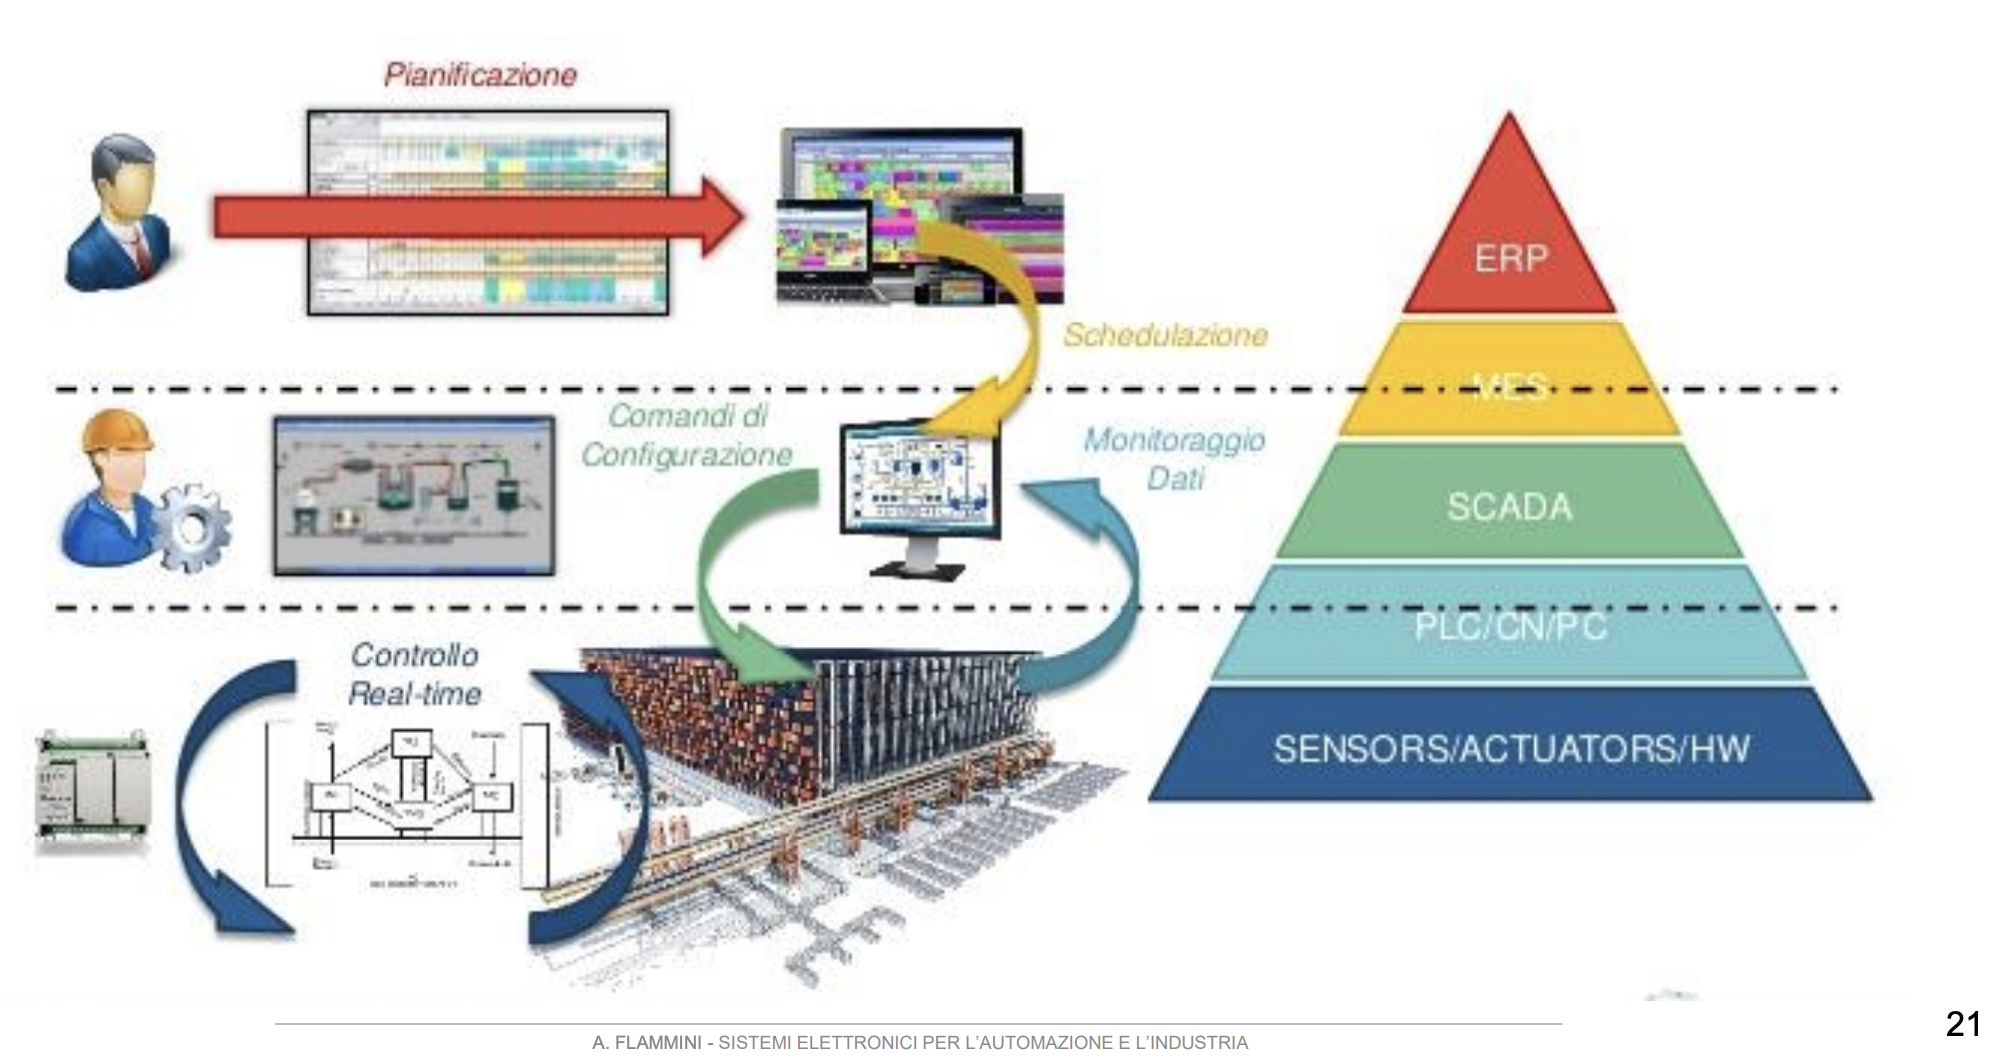
\includegraphics[width=0.5\linewidth]{cim3.png}
    \caption{Computer Integrated Manufacturing}
\end{figure}
\begin{figure}
    \centering
    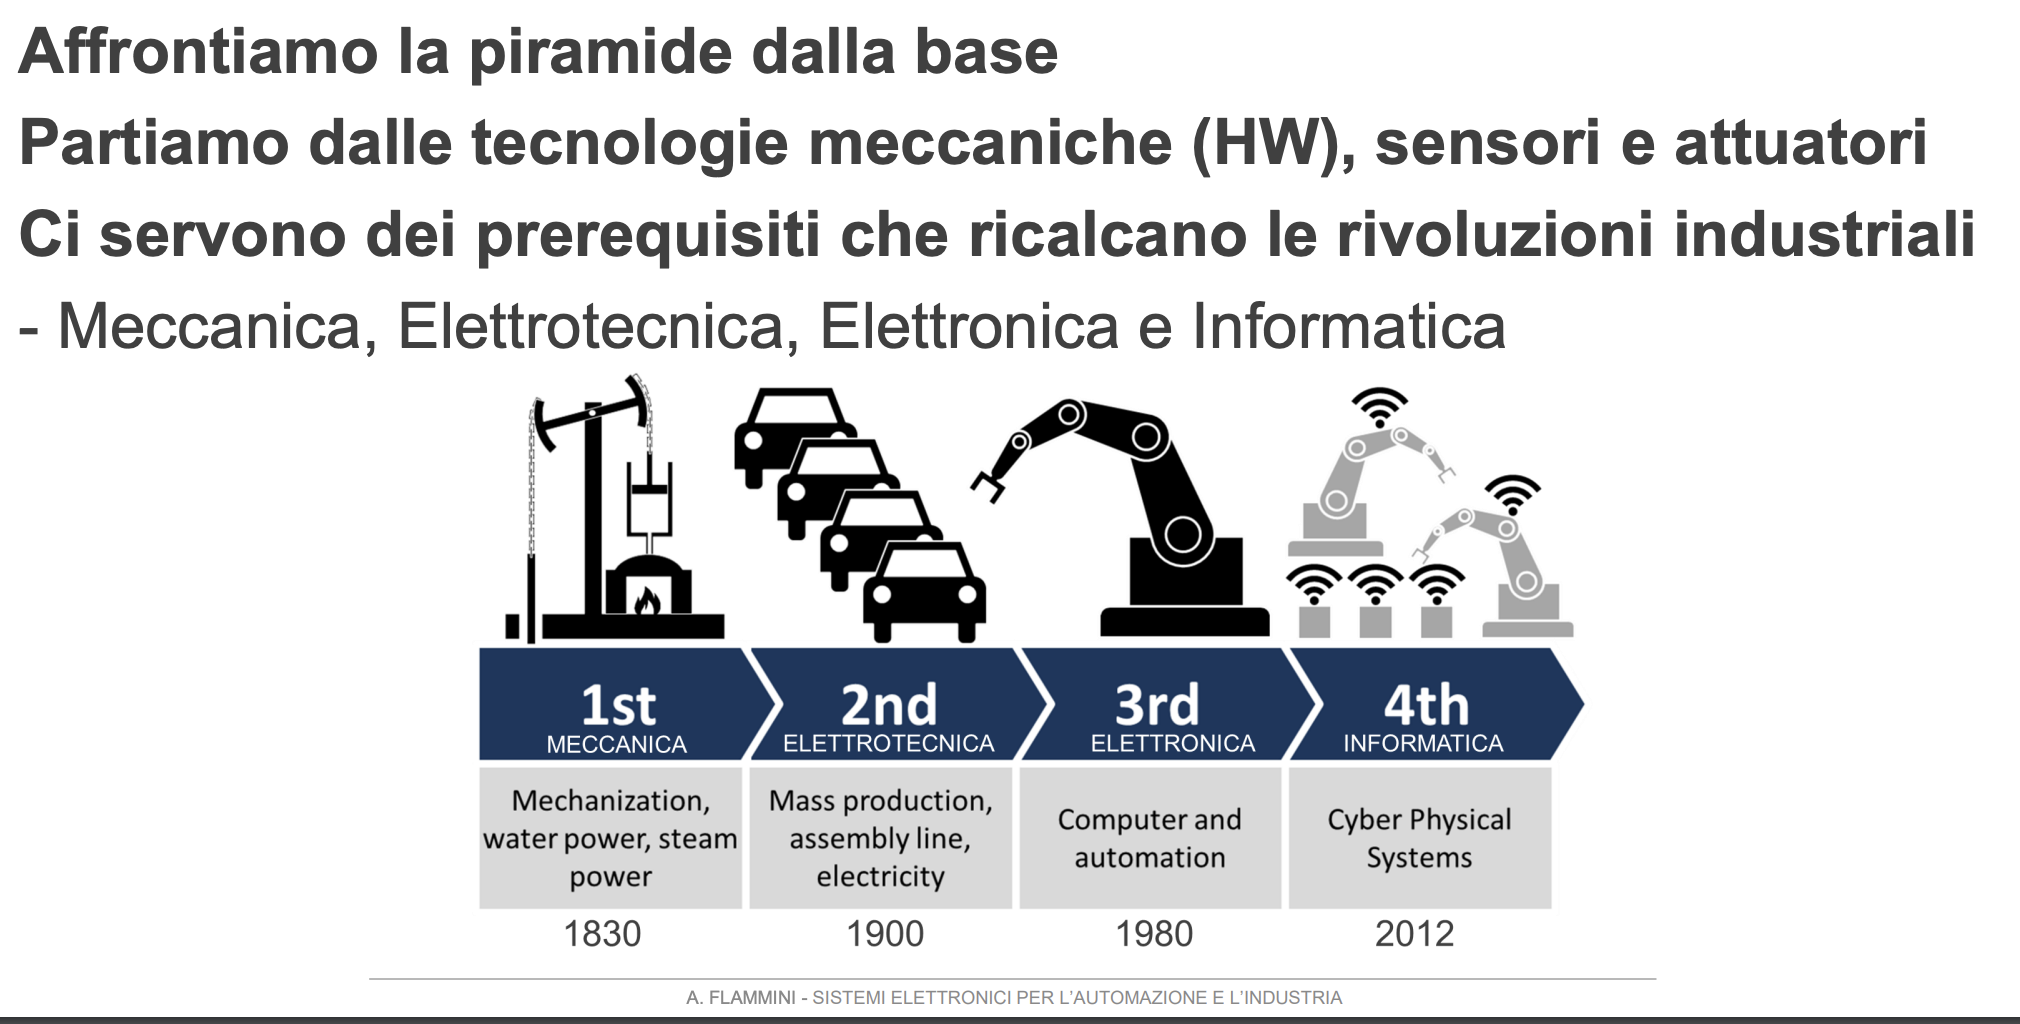
\includegraphics[width=0.5\linewidth]{cim4.png}
    \caption{Computer Integrated Manufacturing}
\end{figure}

\section{Solo menzionati}
\subsection{Lean production}
Inventata dai Giapponesi. AVEVO LA LEAN NEL BACK
\begin{figure}[h!]
    \centering
    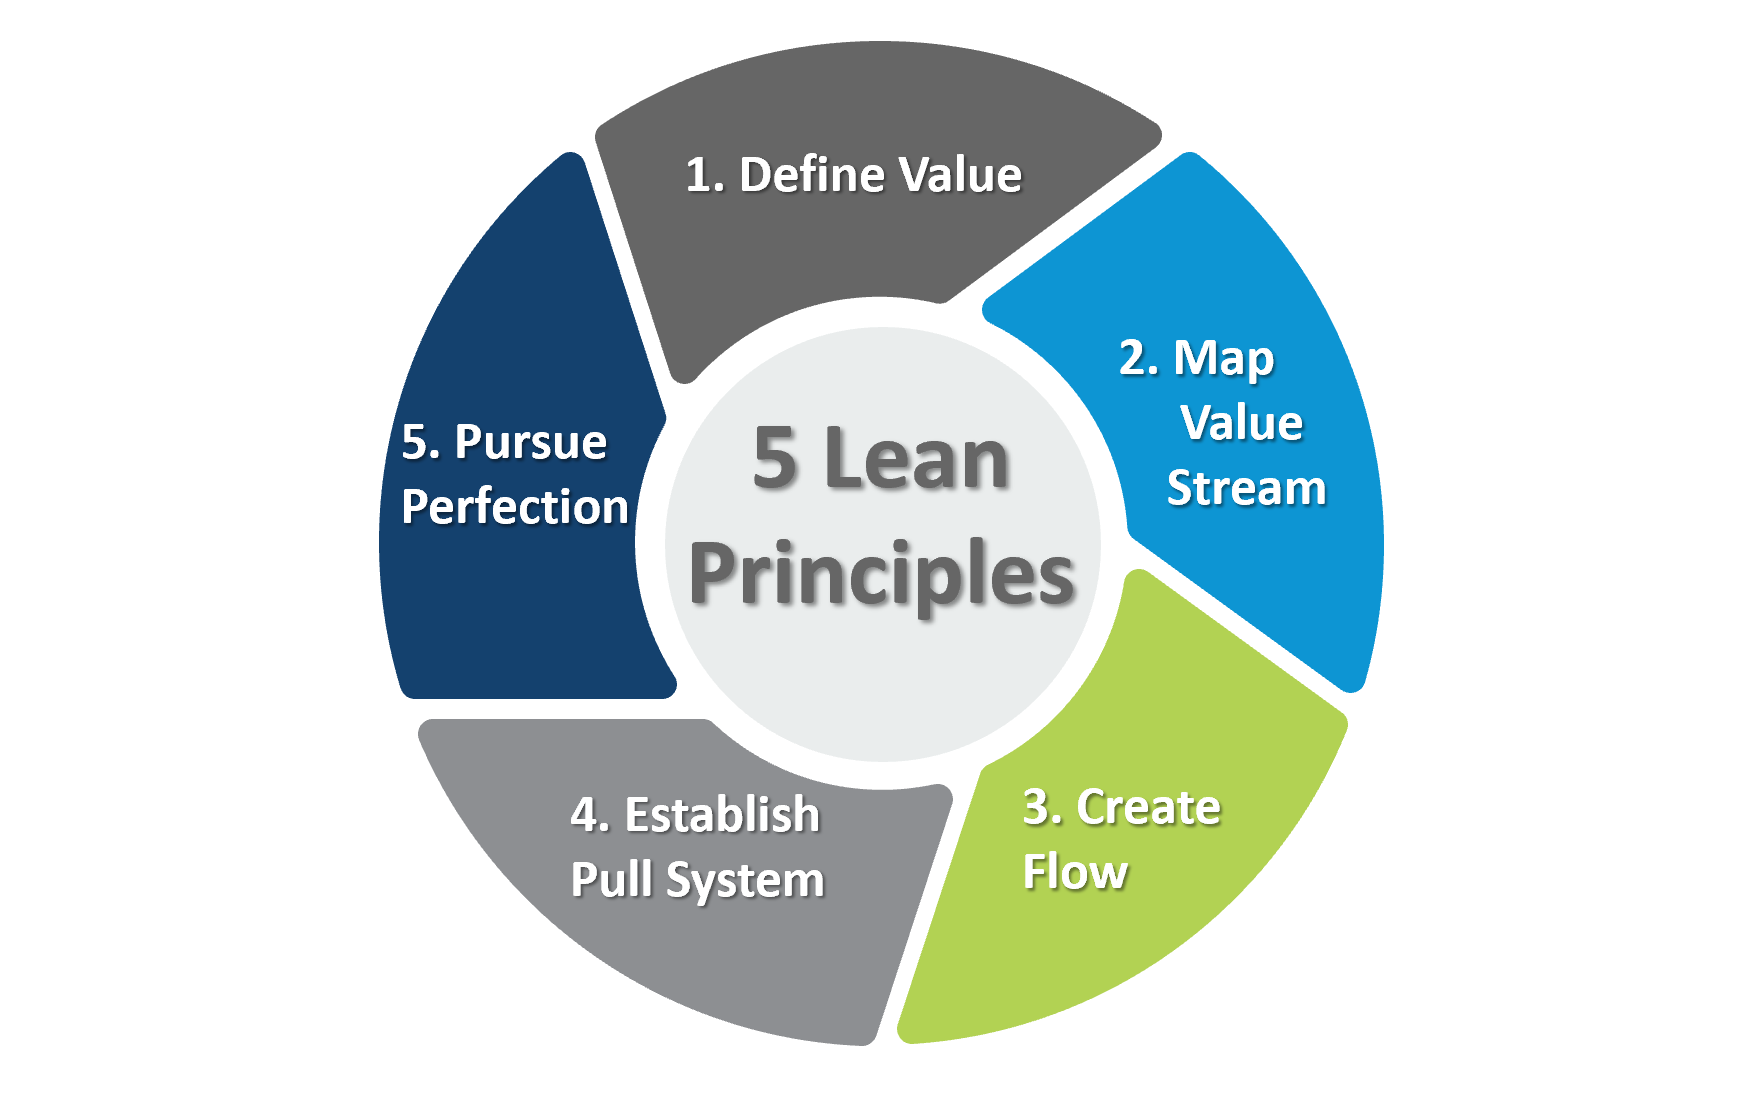
\includegraphics[width=0.5\linewidth]{lean.png}
    \caption{Lean production}
\end{figure}

\subsection{Tecnologie abilitanti di industria 5.0}
\begin{enumerate}
    \item \textbf{Introduction}
        \begin{itemize}
            \item 1.1 The concept of Industry 5.0
            \item 1.2 Comments on the term and concept of Industry 5.0
        \end{itemize}
    \item \textbf{Enabling technologies}
        \begin{itemize}
            \item 2.1 Individualised Human-machine-interaction
            \item 2.2 Bio-inspired technologies and smart materials
            \item 2.3 Digital twins and simulation
            \item 2.4 Data transmission, storage, and analysis technologies
            \item 2.5 Artificial Intelligence
            \item 2.6 Technologies for energy efficiency, renewables, storage and autonomy
        \end{itemize}
    \item \textbf{Challenges and Enablers}
        \begin{itemize}
            \item 3.1 Social dimension
            \item 3.2 Governmental and political dimension
            \item 3.3 Interdisciplinarity
            \item 3.4 Economic dimension
            \item 3.5 Scalability
        \end{itemize}
\end{enumerate}







\end{document}